% ──────────────────────────────────────────────────────────────────
%  NeSy-Mamba: Slot-Gated State Space Models for Interpretable
%  Logical Reasoning
%  IEEE Conference Format
% ──────────────────────────────────────────────────────────────────
\documentclass[conference]{IEEEtran}

% ── Packages ──────────────────────────────────────────────────────
\usepackage{amsmath,amssymb,amsfonts}
\usepackage{algorithmic}
\usepackage{algorithm}
\usepackage{graphicx}
\usepackage{textcomp}
\usepackage{xcolor}
\usepackage{booktabs}
\usepackage{multirow}
\usepackage{hyperref}
\usepackage{enumitem}
\usepackage{float}
\usepackage{tikz}
\usepackage{pgfplots}
\pgfplotsset{compat=newest}
\usepgfplotslibrary{groupplots}
\usetikzlibrary{positioning, arrows.meta, fit, calc, decorations.pathreplacing}

\definecolor{mamba}{RGB}{52,101,164}
\definecolor{slot}{RGB}{204,102,0}
\definecolor{lossred}{RGB}{164,0,0}
\definecolor{embed}{RGB}{78,154,6}
\definecolor{headpurp}{RGB}{117,80,123}
\definecolor{mono}{RGB}{204,0,0}
\definecolor{ema_unsup}{RGB}{52,101,164}
\definecolor{ema_sup}{RGB}{78,154,6}

% ── Macros ────────────────────────────────────────────────────────
\DeclareRobustCommand{\model}{NeSy-Mamba}
\newcommand{\Real}{\mathbb{R}}
\newcommand{\sigmoid}{\sigma}
\newcommand{\softmax}{\mathrm{softmax}}
\newcommand{\ie}{\textit{i.e.}}
\newcommand{\eg}{\textit{e.g.}}
\newcommand{\cf}{\textit{cf.}}
\newcommand{\etal}{\textit{et~al.}}
\newcommand{\wrt}{w.r.t.}

% Draft helpers (no-ops for camera-ready; restore for review)
\newcommand{\todo}[1]{}
\newcommand{\placeholder}[1]{}

\begin{document}

% ══════════════════════════════════════════════════════════════════
\title{NeSy-Mamba: Slot-Gated State Space Models\\for Interpretable Logical Reasoning}

\author{
    \IEEEauthorblockN{Samarth Bhalerao}
    \IEEEauthorblockA{
        \textit{Dept.\ of Electronics and Telecommunication} \\
        \textit{Vishwakarma Institute of Information Technology} \\
        Pune, India \\
        samarth.22211024@viit.ac.in
    }
}

\maketitle

% ══════════════════════════════════════════════════════════════════
\begin{abstract}
Can a 273K-parameter model reason over logical rules---and explain
itself while doing so? We tackle this question with \model{}, an
architecture that grafts symbolic slot gates onto Mamba, a selective
state space model running in $O(L)$ time. Each of $K$ slots
tracks whether a particular class of logical rule has fired,
producing a soft proof trajectory that evolves token by token.
The key mechanism is an \emph{exponential moving average (EMA)
gate} whose memory coefficient is itself input-dependent: slots
can hold onto accumulated evidence or revise their beliefs,
much like a GRU update gate---except here the gated quantities
are interpretable truth flags, not opaque hidden units.

We also contribute a \emph{rule-type taxonomy} that sorts
ProofWriter rules into seven semantic bins (propositional
implication, conjunction, relational chaining, among others)
by tracing proof provenance, and we use the resulting
multi-hot labels to supervise the slots during training.

On ProofWriter (118K examples, depths 0--5), the supervised
model reaches $80.3 \pm 0.4\%$ validation accuracy across seeds.
That number alone is unremarkable---RuleTaker hits $\sim$99\%
with 460$\times$ more parameters~\cite{clark2020ruletaker}. What
caught our attention was the variance story. Unsupervised runs
swing by $\pm6.3$--$6.6$~pp from seed to seed; supervision
crushes that to $\pm0.4$~pp, a $16\times$ reduction. Symbolic
slot labels, it turns out, do double duty: they make the model
interpretable \emph{and} anchor its training dynamics, acting
less like an annotation convenience and more like a structural
regulariser. Code and checkpoints are available publicly.
\end{abstract}

\begin{IEEEkeywords}
neuro-symbolic AI, state space models, Mamba, interpretable
reasoning, logical inference, slot-gated networks
\end{IEEEkeywords}

% ══════════════════════════════════════════════════════════════════
\section{Introduction}
\label{sec:intro}

Start with a concrete scenario. You have the fact ``The cat is blue''
and the rule ``If something is blue then it is kind.'' A competent
reasoning engine should derive ``The cat is kind.'' Straightforward
enough---but stack two, three, or five such steps together, and the
task demands that the model hold intermediate conclusions in memory and
compose them without error. That is \emph{multi-hop} logical reasoning,
and it remains a hard test of systematic
generalisation~\cite{clark2020ruletaker}.

Symbolic systems---Prolog, answer set solvers---handle this natively
through unification and resolution, with soundness and completeness
baked in. Their weakness is brittleness: reword a fact slightly, and
the whole inference chain can break. Neural models sit at the other
extreme. Fine-tuned Transformers score above 95\% on ProofWriter, but
ask them \emph{which} rules they used and in what order, and you get
silence~\cite{tafjord2021proofwriter}.

The neuro-symbolic community has tried to bridge this gap from multiple
angles. DeepProbLog~\cite{manhaeve2018deepproblog} embeds neural outputs
into probabilistic logic programs.  Logic Tensor
Networks~\cite{badreddine2022ltn} ground first-order logic in
differentiable tensors.  Concept bottleneck
models~\cite{koh2020cbm} and retrieval-augmented LLM
pipelines~\cite{kazemi2023lambada} each contribute something
different. But two things stay constant across these methods: they all
sit on top of Transformer backbones (with $O(L^2)$ attention), and any
interpretability they offer is an afterthought---bolted on via proof
decoders, chain-of-thought prompts, or attention heatmaps, not woven
into the core computation.

\subsection{The Interpretability Gap}

How well do existing neural provers actually work? Very well, on
benchmarks.  RuleTaker~\cite{clark2020ruletaker} fine-tunes
RoBERTa-large (125M parameters) and reaches $\sim$99\% accuracy on
ProofWriter. PRover~\cite{saha2020prover} adds proof graph generation
at comparable accuracy.  The numbers are impressive.  The problem is
what happens when you try to look inside.

Post-hoc explanation tools---attention
visualisation~\cite{jain2019attention}, LIME, SHAP, integrated
gradients~\cite{sundararajan2017ig}---all approximate. They rarely
correspond to the computation the model actually performed, and Jain
and Wallace~\cite{jain2019attention} showed that attention weights
in particular can be misleading. So the question becomes: is it
possible to build a model that explains itself \emph{by design}---one
whose internal state directly encodes which rules fired and when,
without any bolt-on probes? That is the kind of interpretability we
are after.

\subsection{The Efficiency Gap}

Self-attention costs $O(L^2)$ in sequence length. For ProofWriter,
where sequences average 63 tokens, this is a non-issue. Scale up to
knowledge bases with hundreds of facts, though, and the arithmetic
changes fast: $O(63^2) \approx 4$K vs.\ $O(1000^2) = 1$M.

Mamba~\cite{gu2023mamba}, a selective state space model, processes
sequences in $O(L)$ by making the SSM parameters ($\Delta_t$, $B_t$,
$C_t$) functions of the current token. The model decides, token by
token, how much to absorb versus how much to forget---a kind of
content-based gate that, in practice, matches Transformer-level
language modelling quality at a fraction of the cost. Nobody, however,
has tried Mamba on \emph{logical reasoning} tasks.  Our hunch is that
its selective scan is a natural substrate for tracking which rules
become active as the model reads through a theory, provided we add an
explicit symbolic layer on top.

\subsection{Our Approach}

\model{} is built around three pieces that work in concert.
First, a \textbf{Mamba backbone} reads the concatenated
fact+rule+query string in linear time and produces contextualised
hidden states $\mathbf{h}(t)$ at each timestep. Second, a
\textbf{symbolic slot gate} maintains $K$ truth-flag values
$\mathbf{s}(t) \in [0,1]^K$---one per rule class---that track
which rule types the model considers active as it scans the input.
Third, a suite of \textbf{differentiable logic losses} supplies
supervision from proof-provenance labels, enforces answer--slot
consistency, and penalises representational collapse through
orthogonality and entropy terms.

On the technical side, the most important design choice is the
\emph{EMA slot gate} with \emph{dynamic memory coefficients}.
Earlier slot-filling architectures~\cite{bao2022slot} use a
monotonic max gate---once a slot activates, it cannot deactivate.
Section~\ref{sec:analysis} shows where this goes wrong:
every slot ratchets to the same value and carries zero
input-specific information. We replace the max with an exponential
moving average:
\begin{equation}
    s_k(t) = \alpha_k(t) \cdot s_k(t{-}1) + (1 - \alpha_k(t)) \cdot \hat{s}_k(t)
\label{eq:ema_intro}
\end{equation}
where $\alpha_k(t) = \sigma(W_\alpha \cdot h_t + b_{\alpha_k})$
depends on the current hidden state. High $\alpha$ means ``hold
onto what you have''; low $\alpha$ means ``revise.''  Because the
coefficient is input-dependent, the same slot behaves differently at
different positions---sluggish on irrelevant tokens, responsive on
evidence tokens. The analogy with GRU update gates is deliberate;
the difference is that here the gated quantities are interpretable
rule-type flags.

\subsection{Key Finding: Supervision as Stabilisation}

We did not expect the following result. Running three seeds across
four configurations, we found that without type-based slot labels,
accuracy swings by $\pm 6.3$--$6.6$~pp from seed to seed.
With labels ($\lambda_s{=}1.0$), the swing drops to $\pm 0.4$~pp---a
$16\times$ reduction. The gap between our best unsupervised run
(80.6\%) and our worst (65.3\%) is enormous for the same
architecture; supervision eliminates it almost entirely.
The slot labels, designed for interpretability, turn out to function
primarily as a structural regulariser that rescues a small model
from its rugged loss landscape.

\subsection{Contributions}

Concretely, the paper makes five contributions:
\begin{enumerate}[nosep]
    \item \model{} itself---the first system pairing selective SSMs
          with symbolic slot gates for logical reasoning, performing
          multi-hop inference at $O(L)$ cost with built-in
          interpretability.
    \item A diagnosis of \emph{monotonic slot collapse} in max-gated
          neuro-symbolic models, together with the EMA gate
          (dynamic~$\alpha$) as a principled remedy rooted in the
          EMA--GRU correspondence.
    \item A seven-category \emph{rule-type taxonomy} derived from
          ProofWriter proof provenance, producing structured
          multi-hot labels for slot supervision.
    \item Quantitative evidence, from multi-seed ablation, that
          type-based slot supervision cuts cross-seed variance by
          $16\times$ ($\pm 0.4$\% vs.\ $\pm 6.3$--$6.6$\%),
          establishing it as a training stabiliser beyond its
          interpretability role.
    \item Public release of all code, logs, and seed-level results.
\end{enumerate}

Section~\ref{sec:related} surveys related work;
Section~\ref{sec:method} details the architecture;
Sections~\ref{sec:experiments}--\ref{sec:results} cover
experiments and results; Section~\ref{sec:analysis} analyses
slot dynamics; Section~\ref{sec:discussion} discusses
implications; Section~\ref{sec:conclusion} concludes.


% ══════════════════════════════════════════════════════════════════
\section{Related Work}
\label{sec:related}

\subsection{State Space Models for Sequence Modelling}

S4~\cite{gu2022s4} was the paper that changed how people think about
linear recurrences. By initialising the state matrix with HiPPO
coefficients and parameterising it as low-rank-plus-diagonal, Gu
et~al.\ showed that a simple recurrence could match---and sometimes
beat---Transformers on the Long Range Arena. The trick is that
continuous-time state space equations, discretised with the right
step sizes, naturally preserve long-range dependencies; no attention
matrix needed.

Mamba~\cite{gu2023mamba} pushed this further. Its defining move is
to make $\Delta$, $B$, $C$ all functions of the current token, so
the state transition changes at every timestep. The model gets to
decide, on the fly, which tokens to absorb and which to let
through---content-dependent gating at $O(L)$ cost. A hardware-aware
scan kernel makes this practical on GPUs. Since its release, Mamba
has been applied to vision (Vim~\cite{zhu2024vim}, bidirectional
scanning of image patches), DNA modelling~\cite{gu2023mamba}, and
time series forecasting.

Mamba-2 later improved parallelisation via structured masked
attention duality; hybrid Mamba-attention architectures have also
appeared.  But here is the gap: nobody has used Mamba---or any SSM,
for that matter---for \emph{structured symbolic reasoning}. Tasks
where the model must track which logical rules have fired and
compose multi-step proofs are, to the best of our knowledge,
entirely uncharted territory for SSMs.  \model{} is designed
specifically to explore whether Mamba's token-gated recurrence
can serve as the backbone for interpretable logical inference.

\subsection{Neural Theorem Proving}

ProofWriter~\cite{tafjord2021proofwriter} turned logical reasoning
into a binary classification problem: given facts, rules, and a
query, predict entailment. Proof depths run from~0 (fact lookup)
to~5 (five chained steps), which makes it possible to probe
reasoning depth in a controlled way.

The dominant result belongs to RuleTaker~\cite{clark2020ruletaker}:
RoBERTa-large (125M parameters), fine-tuned on theory+query pairs,
hits $\sim$99\% accuracy. PRover~\cite{saha2020prover} gets similar
numbers while also predicting proof graphs---but critically, the
proof output comes from an auxiliary decoder bolted onto the side,
not from the prediction pathway itself.

LAMBADA~\cite{kazemi2023lambada} tries backward chaining with LLMs,
recursively decomposing queries into sub-goals. The reasoning traces
read more naturally, but each step pays the $O(L^2)$ attention
tax, and backward chaining multiplies that by the number of
sub-goals. Chain-of-thought prompting~\cite{wei2022chain} and
selection-inference modules~\cite{creswell2022selection} round out
the landscape.

The shared pattern across all of these systems: Transformer backbone,
quadratic cost, interpretability as an add-on.  We are not trying to
beat their accuracy---273K parameters versus 125M would make that a
strange ambition. The question is narrower: can an SSM backbone with
symbolic slots baked in handle this task at all, and if so, what do
the slots reveal about how the model reasons?

\subsection{Neuro-Symbolic Integration}

The neuro-symbolic landscape is broad, so we focus on the lines of
work closest to ours.

\textbf{Logic programming integration.}
DeepProbLog~\cite{manhaeve2018deepproblog} feeds neural outputs into
ProbLog as probabilistic facts; NeurASP~\cite{yang2020neurasp}
does something analogous with answer set programming. Both give
strong logical guarantees but demand hand-written symbolic programs
and run into differentiability issues at the neural--symbolic
boundary.

\textbf{Differentiable logic.}
Logic Tensor Networks~\cite{badreddine2022ltn} take a different
tack: ground first-order formulas directly in tensor space and
train end-to-end with logical constraints as part of the loss.
Of the existing methods, this is probably the closest cousin to
our differentiable logic losses---the key difference being that
LTN operates on object-level features rather than temporal
sequences of rule activations.

\textbf{Concept bottleneck architectures.}
Concept Bottleneck Models~\cite{koh2020cbm} force predictions
through a layer of human-readable concepts. Our slot gate borrows
the same intuition---each slot is named after a rule type---but it
works sequentially: slot values change over the input, whereas
concept bottleneck features are computed in a single pass.

\textbf{Slot-structured representations.}
Slot Attention~\cite{locatello2020slot} decomposes visual scenes
into object-level slot vectors via iterative attention. The name
is shared, but the substance differs: our slots hold
\emph{truth values of logical rules}, not object features, and
they update via SSM recurrence, not iterative attention.

Where does \model{} sit in all of this? Three things set it apart:
(i)~an SSM backbone rather than attention, (ii)~slots that encode
truth flags rather than object descriptors, and (iii)~temporal EMA
dynamics that record \emph{when} along the input sequence each rule
type became relevant.

\subsection{Gating Mechanisms and Temporal Dynamics}

Our EMA gate borrows from a long line of gating ideas.

\textbf{GRU and LSTM gates.}
The GRU~\cite{cho2014gru} update gate $z_t = \sigma(W_z x_t + U_z
h_{t-1})$ controls how much old information persists. Our per-slot
$\alpha_k(t)$ does the same job, but over interpretable truth flags
rather than dense hidden vectors. Because each slot has a semantic
label, the $\alpha_k(t)$ trajectory is directly readable: you can
see, token by token, when the model starts paying attention to a
particular rule class.

\textbf{Monotonic and irreversible gates.}
The max gate we are replacing resembles the CumMax in Ordered
Neurons (ON-LSTM~\cite{shen2019ordered}). There, irreversibility
is a feature---higher-level constituents should persist. In
reasoning, it is a bug. Once every slot ratchets to the same
ceiling, they all say the same thing regardless of the input.
Section~\ref{sec:analysis} documents this failure in detail.

\textbf{EMA in deep learning.}
Exponential moving averages crop up everywhere---batch norm
running statistics, DQN target networks, BYOL momentum encoders.
The twist in our case is that $\alpha_k(t)$ is learned and
input-dependent, making the gate an adaptive filter. This is not
optional: for reasoning, a slot must hold steady on noise tokens
(high $\alpha$) and snap to attention on evidence tokens
(low $\alpha$).


% ══════════════════════════════════════════════════════════════════
\section{Method}
\label{sec:method}

Three modules make up the architecture (Figure~\ref{fig:architecture}):
a Mamba backbone for sequence encoding
(Section~\ref{sec:backbone}), a symbolic slot gate for tracking
rule activations (Section~\ref{sec:slotgate}), and a set of
differentiable logic losses that provide structured supervision
(Section~\ref{sec:logicloss}).

\begin{figure}[t]
    \centering
    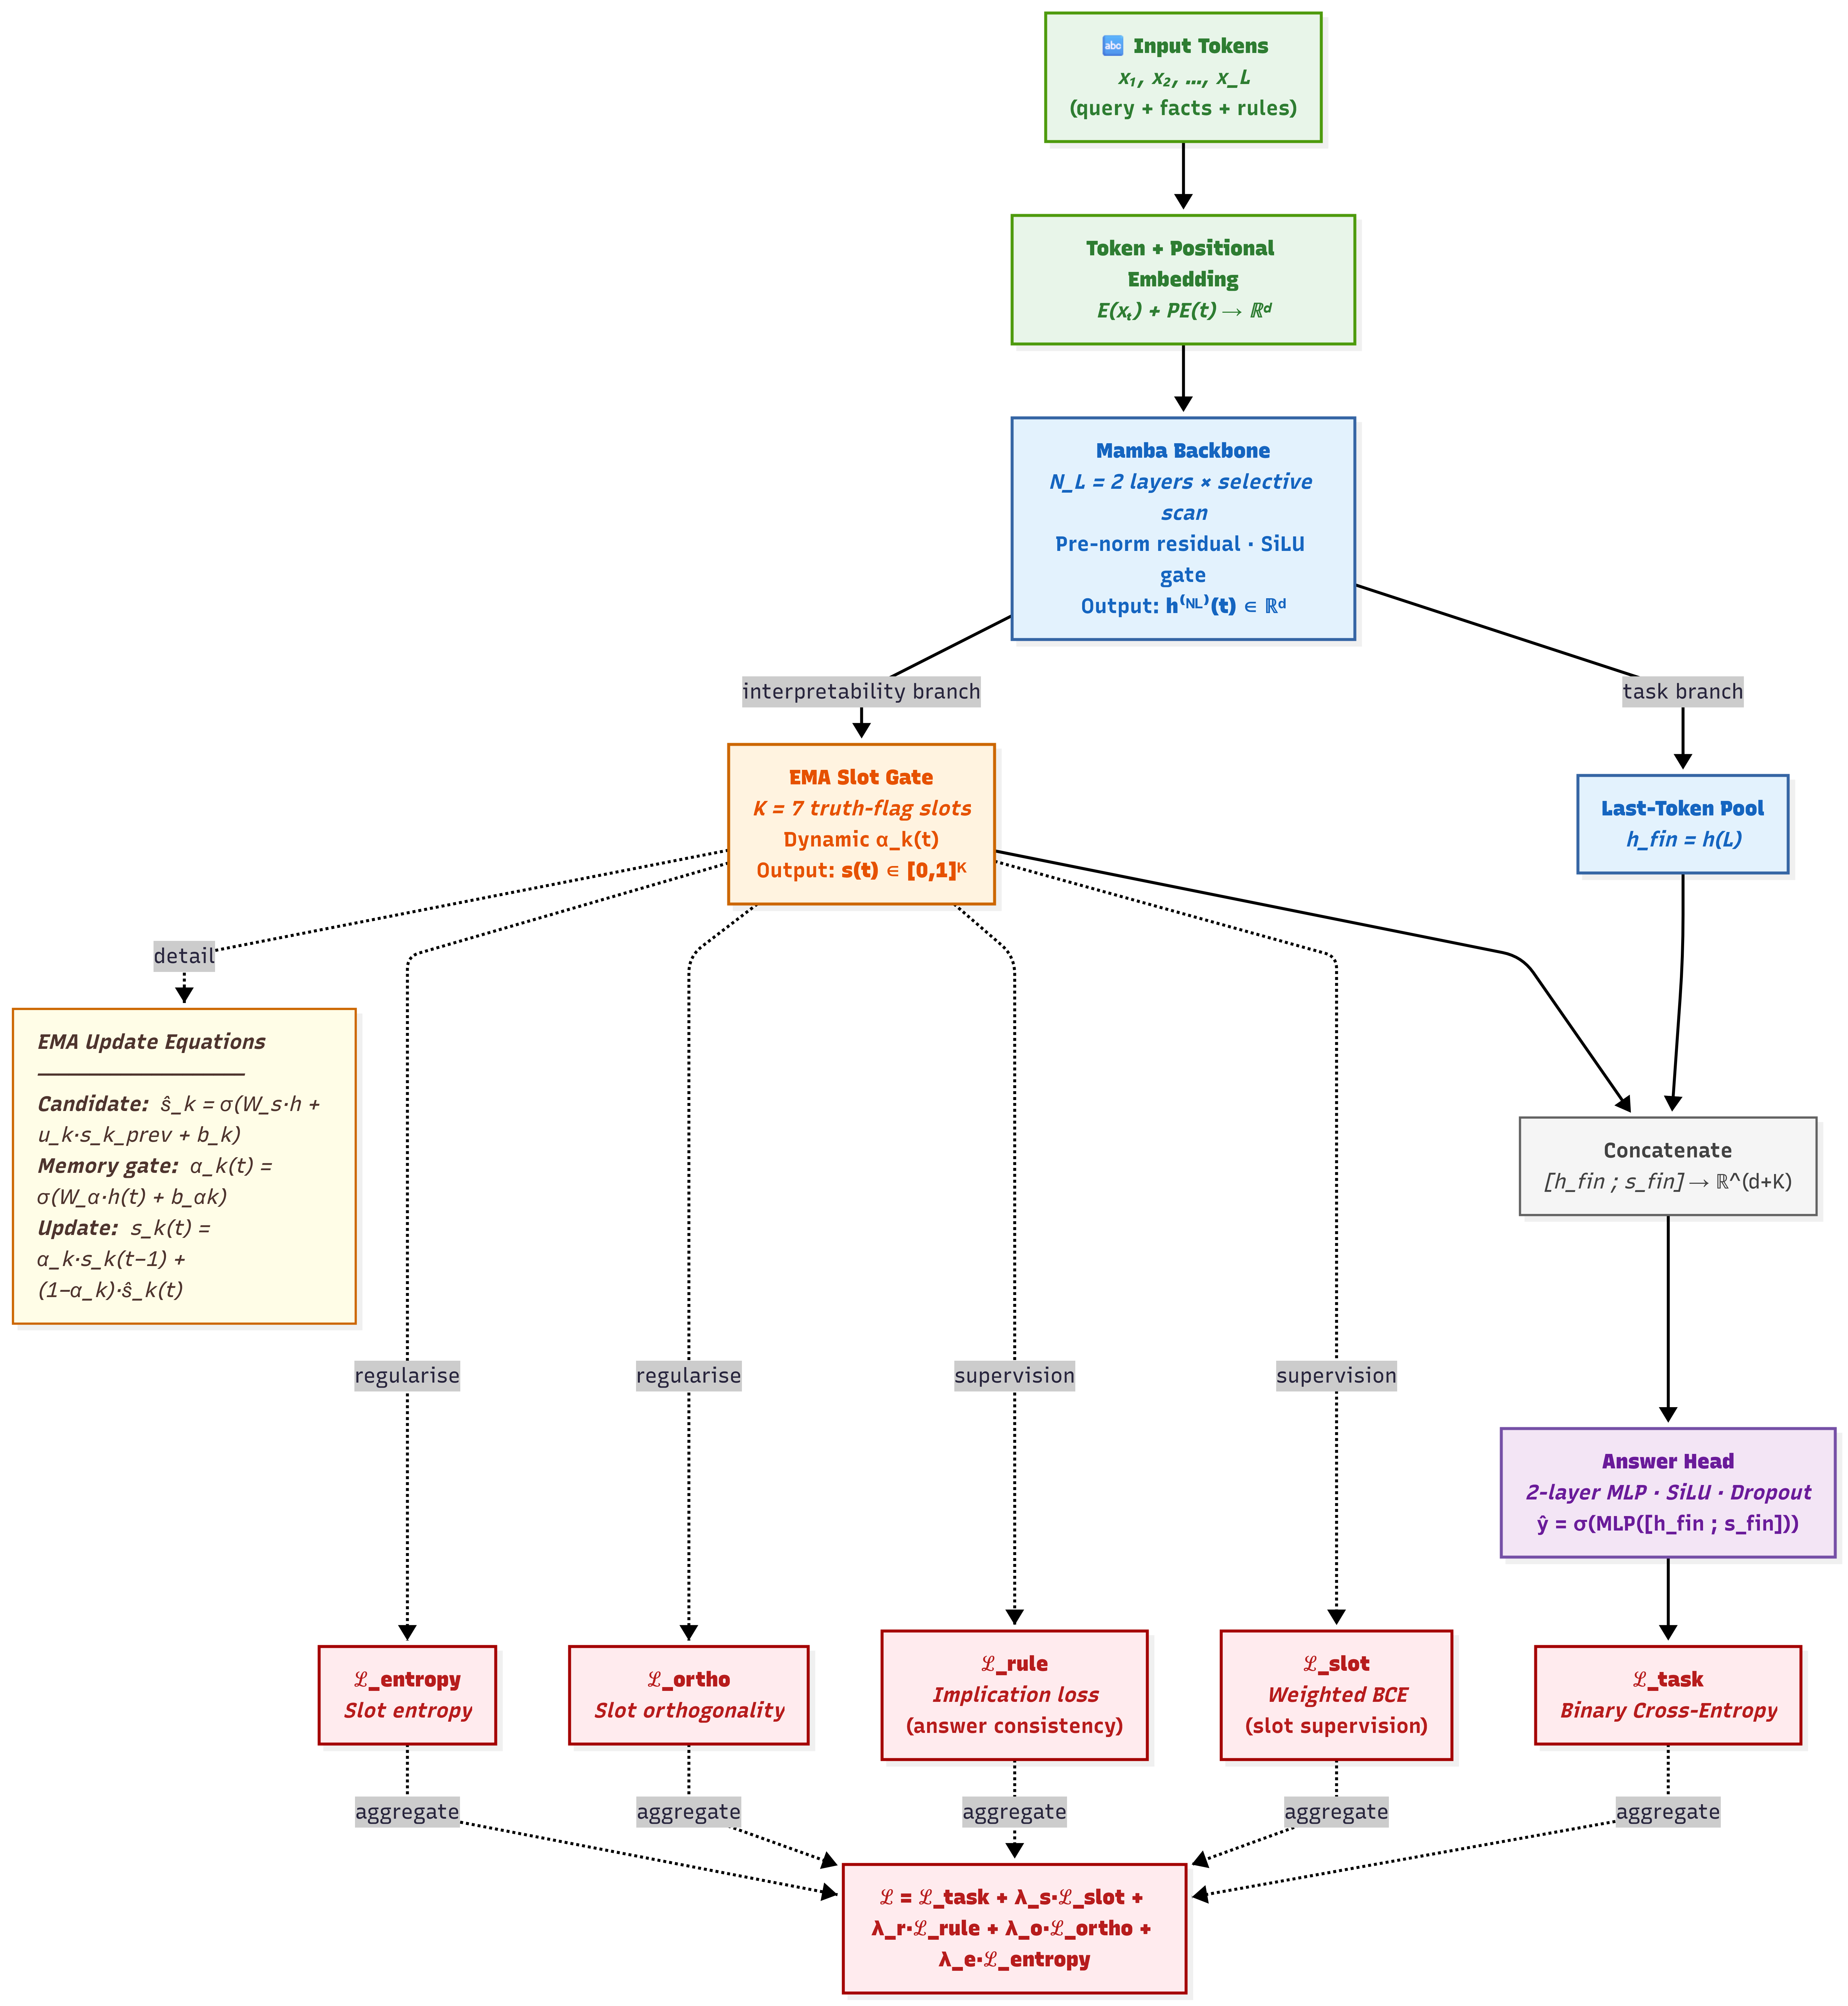
\includegraphics[width=\columnwidth]{architecture.png}
    \caption{\textbf{Architecture of \model{}.}  The Mamba backbone
    reads the tokenised theory+query in $O(L)$ time via
    selective scan.  Hidden states $\mathbf{h}(t)$ branch into
    (i)~last-token pooling for the answer head and (ii)~the EMA
    slot gate, which maintains $K{=}7$ truth-flag
    values $\mathbf{s}(t) \in [0,1]^K$.  The memory
    coefficient $\alpha_k(t)$ is input-dependent, letting each slot
    hold or revise its belief at every timestep.  Five loss terms
    train the system jointly: task BCE, slot supervision,
    answer consistency, orthogonality, and entropy regularisation.
    Dashed arrows = supervision; solid arrows = data flow.}
    \label{fig:architecture}
\end{figure}

In brief, the forward pass proceeds by: tokenising and embedding
the concatenated query+facts+rules string; running $N_L$ Mamba
blocks to produce contextualised hidden states; updating $K$ slot
values at each timestep through the EMA gate; and finally
concatenating the last hidden state with the slot vector to feed
a two-layer MLP that outputs the answer. Four auxiliary losses
act on the slots during training (Algorithm~\ref{alg:forward}).

\begin{algorithm}[t]
\caption{\model{} Forward Pass and Loss Computation}
\label{alg:forward}
\begin{algorithmic}[1]
\REQUIRE Theory+query sequence $x = (x_1, \ldots, x_L)$,
  slot labels $\mathbf{s}^* \in \{0,1\}^K$ (if supervised),
  answer label $y^*$
\STATE \textbf{Embed:} $\mathbf{e}(t) \leftarrow \mathrm{Emb}(x_t) + \mathrm{Pos}(t)$
        for $t = 1, \ldots, L$
\STATE \textbf{Mamba:} $\mathbf{h}^{(0)}(t) \leftarrow \mathbf{e}(t)$
\FOR{$l = 1$ to $N_L$}
    \STATE $\mathbf{h}^{(l)} \!\leftarrow\! \mathbf{h}^{(l-1)} \!+\!
        \mathrm{Drop}(\mathrm{Mamba}^{(l)}(\mathrm{RMSNorm}(\mathbf{h}^{(l-1)})))$
\ENDFOR
\STATE \textbf{Slot Gate:} Initialise $\mathbf{s}(0) \leftarrow \mathbf{0}$
\FOR{$t = 1$ to $L$}
    \STATE $\hat{s}_k(t) \leftarrow \sigma(W_s \mathbf{h}^{(N_L)}(t) + u_k s_k(t{-}1) + b_k)$ for each $k$
    \STATE $\alpha_k(t) \leftarrow \sigma(W_\alpha \mathbf{h}^{(N_L)}(t) + b_{\alpha_k})$
    \STATE $s_k(t) \leftarrow \alpha_k(t) \cdot s_k(t{-}1) + (1-\alpha_k(t)) \cdot \hat{s}_k(t)$
\ENDFOR
\STATE \textbf{Pool:} $\mathbf{h}_{\mathrm{fin}} \leftarrow \mathbf{h}^{(N_L)}[\ell-1]$ \COMMENT{last real token}
\STATE \textbf{Predict:} $\hat{y} \leftarrow \sigma(\mathrm{MLP}([\mathbf{h}_{\mathrm{fin}}; \mathbf{s}(L)]))$
\STATE \textbf{Losses:}
\STATE $\quad \mathcal{L}_{\text{task}} \leftarrow \mathrm{BCE}(\hat{y}, y^*)$
\STATE $\quad \mathcal{L}_{\text{slot}} \leftarrow \text{WeightedBCE}(\mathbf{s}(L), \mathbf{s}^*)$
\STATE $\quad \mathcal{L}_{\text{rule}} \leftarrow \text{AnswerConsistency}(\mathbf{s}(L), \hat{y})$
\STATE $\quad \mathcal{L}_{\text{ortho}} \leftarrow \|{\hat{S}^\top \hat{S} - I_K}\|_F$
\STATE $\quad \mathcal{L}_{\text{entropy}} \leftarrow \text{SlotEntropy}(\mathbf{s})$
\STATE $\quad \mathcal{L} \leftarrow \mathcal{L}_{\text{task}} + \lambda_s \mathcal{L}_{\text{slot}} + \lambda_r \mathcal{L}_{\text{rule}} + \lambda_o \mathcal{L}_{\text{ortho}} + \lambda_e \mathcal{L}_{\text{entropy}}$
\RETURN $\hat{y}$, $\mathbf{s}(1), \ldots, \mathbf{s}(L)$, $\mathcal{L}$
\end{algorithmic}
\end{algorithm}

\subsection{Input Representation}
\label{sec:input}

Each input consists of a theory $\mathcal{T} = \{f_1, \dots, f_M,
r_1, \dots, r_N\}$ of facts and rules expressed in natural
language, together with a query~$q$. These are concatenated into
a single input sequence $x$:
\begin{equation}
    x = [q\ ;\ f_1\ ;\ \dots\ ;\ f_M\ ;\ r_1\ ;\ \dots\ ;\ r_N]
\end{equation}
We place the query first so the Mamba backbone can condition its
selective scan on the information need before it encounters the
full theory---similar to the ``question-first'' ordering used in
reading comprehension models. Structural separator tokens
(\texttt{[FACT]}, \texttt{[RULE]}, \texttt{[SEP]}) are inserted
between segments to mark segment boundaries explicitly.

Tokenisation uses a punctuation-aware splitter that segments on
whitespace and punctuation, yielding a vocabulary of just 41
unique tokens for ProofWriter. This compact vocabulary reflects
the controlled language of the benchmark---entities like
``cat,'' ``dog''; properties like ``blue,'' ``kind''; logical
connectives like ``if,'' ``then,'' ``and.''

Token and learned positional embeddings are summed:
$\mathbf{e}(t) = \mathrm{Emb}(x_t) + \mathrm{Pos}(t)$,
followed by dropout ($p = 0.1$). Positional embeddings are
learned rather than sinusoidal, initialised from
$\mathcal{N}(0, 0.02)$, with a maximum length of 256 tokens---
sufficient for all ProofWriter examples, whose longest sequence
is 194 tokens.

\textbf{Padding and masking.} Variable-length sequences within
a batch are right-padded to the maximum length, and a binary
mask $\mathbf{m} \in \{0,1\}^{L_{\max}}$ is maintained. The
Mamba scan ignores padded positions via masking in the output
projection, and last-token pooling indexes the final non-padded
position per example.

\subsection{Mamba Backbone}
\label{sec:backbone}

The embedded sequence is passed through a stack of $N_L = 2$ Mamba
blocks with pre-norm residual connections:
\begin{equation}
    \mathbf{h}^{(l)} = \mathbf{h}^{(l-1)} +
    \mathrm{Dropout}\!\left(\mathrm{Mamba}\!\left(
    \mathrm{RMSNorm}(\mathbf{h}^{(l-1)})\right)\right)
\end{equation}
We use RMSNorm~\cite{zhang2019rms} rather than LayerNorm for
marginal computational savings and, in our experience, more
stable training dynamics.

\subsubsection{Internal Mamba Block Architecture}

Each Mamba block comprises four stages:
\begin{enumerate}[nosep]
    \item \textbf{Double projection:} A linear layer expands
          from $d_{\text{model}}$ to $2d_{\text{inner}}$ (expand
          factor~2, so $d_{\text{inner}} = 256$). The output is
          split into branch~$\mathbf{x}_B$, which enters the SSM
          pathway, and gate~$\mathbf{z}$, which modulates the output;
    \item \textbf{Causal convolution:} A depth-wise 1-D convolution
          with kernel size $d_c = 4$ and causal padding is applied
          to $\mathbf{x}_B$, followed by SiLU activation. This
          short-range mixing provides a local inductive bias that
          complements the SSM's long-range dynamics;
    \item \textbf{Selective state space recurrence:} The core
          computation distinguishing Mamba from earlier SSMs.
          Discretisation parameters ($\Delta_t$, $B_t$, $C_t$)
          are computed as linear projections of the current token,
          making state transitions \emph{content-dependent};
    \item \textbf{Gated output:} The SSM output is multiplied
          element-wise with $\mathrm{SiLU}(\mathbf{z})$ and
          projected back to $d_{\text{model}}$:
          $\mathbf{y} = (\mathbf{y}_{\text{SSM}} \odot
          \mathrm{SiLU}(\mathbf{z})) \cdot W_{\text{out}}$.
\end{enumerate}

\subsubsection{Selective Scan Mechanism}

The selective SSM discretises continuous-time parameters into
recurrence coefficients:
\begin{align}
    \bar{A}_t &= \exp(\Delta_t \cdot A) \label{eq:disc_a} \\
    \bar{B}_t &= \Delta_t \cdot B_t \label{eq:disc_b} \\
    h_t &= \bar{A}_t \cdot h_{t-1} + \bar{B}_t \cdot x_t
    \label{eq:ssm_recurrence} \\
    y_t &= C_t \cdot h_t + D \cdot x_t \label{eq:ssm_output}
\end{align}
where $A \in \Real^{D \times N}$ is initialised in log-space
using a HiPPO-inspired scheme that promotes long-range signal
propagation. The state dimension $N = d_{\text{state}} = 16$
provides a compact but sufficient latent representation.

The key to Mamba's selectivity is that $\Delta_t$ governs
\emph{how much} of the current token gets absorbed into the state:
large $\Delta_t$ makes $\bar{A}_t \approx 0$ (forget the past,
absorb the input), while small $\Delta_t$ makes $\bar{A}_t
\approx I$ (retain the past, largely ignore the input). For
logical reasoning, this matters: the model can learn to
``attend'' to rule-relevant tokens (``if,'' ``then,'' entity
names) while gliding past filler tokens (``is,'' ``the'').

The step size $\Delta_t$ is computed via a low-rank projection:
$\Delta_t = \mathrm{softplus}(W_{\Delta} \cdot x_t + b_\Delta)$,
where $W_\Delta \in \Real^{d_{\text{inner}} \times d_\Delta}$
(rank $d_\Delta = 2$) followed by broadcast. The softplus
enforces positivity. The bias $b_\Delta$ is initialised via the
inverse-softplus uniform scheme of~\cite{gu2023mamba}, maintaining
stable dynamics during early training.

\subsubsection{Last-Token Pooling}

The final hidden state is obtained via last-real-token pooling:
$\mathbf{h}_{\text{final}} = \mathbf{h}^{(N_L)}[\ell_i - 1]$
where $\ell_i$ is the number of non-padding tokens in example $i$.
This is a natural choice given the causal nature of the SSM: the
last token's hidden state has seen the entire sequence, since the
recurrence propagates information strictly forward in time. Unlike
bidirectional encoders (\eg{} BERT's \texttt{[CLS]} token),
unidirectional pooling introduces an ordering dependence, which
we mitigate by placing the query first in the input sequence.

\subsection{Symbolic Slot Gate}
\label{sec:slotgate}

The slot gate maintains $K$ scalar truth-flag values
$\mathbf{s}(t) = [s_1(t), \dots, s_K(t)] \in [0,1]^K$ that are
updated at every timestep. Each slot represents the model's
soft belief that a particular class of logical rule has fired.

\subsubsection{Candidate Computation}

At each timestep $t$, a candidate activation is computed for each
slot:
\begin{equation}
    \hat{s}_k(t) = \sigma\!\left(
    \underbrace{W_s \cdot \mathbf{h}(t)}_{\text{input-dependent}}
    + \underbrace{u_k \cdot s_k(t{-}1)}_{\text{recurrence}}
    + \underbrace{b_k}_{\text{bias}}
    \right)
\label{eq:candidate}
\end{equation}
where $W_s \in \Real^{K \times d}$ is a shared projection
(Xavier init with gain $g_s$), $u_k$ is a per-slot diagonal
recurrence weight, and $b_k$ is a per-slot bias. We use a
diagonal recurrence---rather than a full $K \times K$
coupling---to preserve per-slot identity and keep the
representation interpretable.

\subsubsection{Optional Slot Competition}

To encourage specialisation---ideally, one dominant slot per
timestep---we optionally apply temperature-scaled softmax
competition:
\begin{equation}
    \tilde{s}_k(t) = \frac{\exp(\hat{s}_k(t) / \tau)}
    {\sum_{j=1}^K \exp(\hat{s}_j(t) / \tau)} \cdot \hat{s}_k(t)
\label{eq:competition}
\end{equation}
where $\tau$ is a temperature hyperparameter.

\subsubsection{Gate Update: Monotonic Max vs. EMA}

\textbf{Monotonic max (baseline).}
The original gate accumulates evidence irreversibly:
\begin{equation}
    s_k(t) = \max\!\left(s_k(t{-}1),\ \tilde{s}_k(t)\right)
\label{eq:monotonic}
\end{equation}
This models proof accumulation (a deduced fact remains
deduced), but it prevents the model from learning from
\emph{negative evidence} and causes all slots to converge
to the same value---as we show in Section~\ref{sec:analysis}.

\textbf{EMA gate (proposed).}
We replace the monotonic max with an exponential moving average:
\begin{equation}
    s_k(t) = \alpha_k(t) \cdot s_k(t{-}1) +
    (1 - \alpha_k(t)) \cdot \tilde{s}_k(t)
\label{eq:ema}
\end{equation}
The memory coefficient $\alpha_k(t)$ controls the balance
between retaining the previous slot value (memory) and
incorporating the new candidate (update).

\textbf{Dynamic $\alpha$ (full model).}
We make $\alpha$ input-dependent via a learned linear projection:
\begin{equation}
    \alpha_k(t) = \sigma\!\left(
    W_\alpha \cdot \mathbf{h}(t) + b_{\alpha_k}
    \right)
\label{eq:dynamic_alpha}
\end{equation}
where $W_\alpha \in \Real^{K \times d}$ is initialised with small
gain (0.1) and the biases $b_{\alpha_k}$ are stagger-initialised
around a high base value ($\sigma(2.0) \approx 0.88$) for symmetry
breaking. This makes each slot a \emph{learnable symbolic filter}:
the model decides per-token how much each slot should hold onto
its current belief versus update from new evidence. This is
analogous to the GRU~\cite{cho2014gru} update gate, but applied
to symbolic truth-flag slots rather than dense hidden states.

\textbf{Static $\alpha$ (ablation).}
For ablation purposes, we also implement a static variant in which
each slot has a single learnable $\alpha_k = \sigma(\ell_k)$
that does not depend on the input. This isolates the contribution
of input-dependence from the EMA mechanism itself.

\subsubsection{Initialisation Strategy}
\label{sec:init}

Getting the initialisation right is critical for avoiding early
collapse. The following strategy was arrived at through systematic
ablation over initialisation schemes:

\begin{itemize}[nosep]
    \item \textbf{Slot projection $W_s$:} Xavier uniform with
          gain $g_s = 1.0$. Lower gains (\eg{} $g_s = 0.1$)
          suppress the input signal relative to the bias,
          causing the bias to dominate and all slots to collapse
          to the same fixed point. This turned out to be the root
          cause of collapse in our early experiments
          (Section~\ref{sec:analysis}).
    \item \textbf{Recurrence weights $u_k$:} Initialised to
          $+0.01$ (small positive). This provides a mild
          self-reinforcing tendency---slots that activate tend
          to stay active, capturing the ``accumulation of evidence''
          intuition. Negative values cause oscillation; large
          positive values lead to runaway activation.
    \item \textbf{Bias $b_k$:} All zeros. Combined with
          $\sigma(0) = 0.5$, this centres the initial candidates
          around 0.5, and the EMA dynamics then push slots toward
          their learned equilibria.
    \item \textbf{Alpha projection $W_\alpha$:} Xavier uniform
          with small gain (0.1). The small gain ensures that early
          in training, $\alpha_k(t) \approx \sigma(b_{\alpha_k})$
          for all tokens, so the gate begins in a near-static
          regime and gradually learns to differentiate.
    \item \textbf{Alpha biases $b_{\alpha_k}$:} Stagger-initialised
          around a high base value. Specifically,
          $b_{\alpha_k} = 2.0 + 0.05 \cdot k$ for
$k \in \{0, \ldots, K{-}1\}$, giving
          $\alpha_k(0) \in [0.88, 0.89]$. The high initial
          $\alpha$ makes slots ``sticky'' at startup (strong
          memory, slow update), preventing rapid collapse into
          degenerate fixed points. The staggering breaks symmetry
          so that different slots start with slightly different
          temporal dynamics.
\end{itemize}

\subsubsection{Firing Order Tracking}

We track the timestep at which each slot first crosses the
activation threshold~$\theta$:
\begin{equation}
    \text{fire}_k = \min\{t : s_k(t) > \theta\}
\end{equation}
This produces a temporal ordering over rule activations that
serves as a proxy for the proof execution trace.

\subsection{Answer Head}
\label{sec:answer}

The final prediction concatenates the Mamba output and slot values
into a joint representation:
\begin{equation}
    \hat{y} = \sigma\!\left(\mathrm{MLP}\!\left(
    [\mathbf{h}_\text{final}\ ;\ \mathbf{s}_\text{final}]
    \right)\right)
\end{equation}
The MLP uses two fully connected layers:
\begin{align}
    \mathbf{z}_1 &= \mathrm{SiLU}\!\left(W_1 [\mathbf{h}_{\text{final}}; \mathbf{s}_{\text{final}}] + \mathbf{b}_1\right) \\
    \hat{y} &= \sigma\!\left(W_2\, \mathrm{Dropout}(\mathbf{z}_1) + b_2\right)
\end{align}
where $W_1 \in \Real^{d_{\text{model}} \times (d_{\text{model}} + K)}$
and $W_2 \in \Real^{1 \times d_{\text{model}}}$, with intermediate
dimension matching $d_{\text{model}} = 128$. We use SiLU (Swish)
activation rather than ReLU based on preliminary experiments
showing faster convergence. Dropout ($p=0.1$) is applied after
the first layer.

The model is trained with binary cross-entropy (BCE) loss:
\begin{equation}
    \mathcal{L}_{\text{task}} = -\left[y^* \log(\hat{y}) \cdot w_+ + (1 - y^*) \log(1 - \hat{y})\right]
\end{equation}
where $w_+ = N_{\text{neg}} / N_{\text{pos}}$ is the positive
class weight computed from the training set (approximately 0.84
for ProofWriter's 54.4/45.6 class split), which prevents the
model from trivially predicting the majority class.

\textbf{Joint representation advantage.}
By concatenating slot values with the backbone hidden state, the
answer head can draw on both the neural representation (which may
capture patterns not captured by slots) and the symbolic one
(which provides structured, interpretable features). Notably, even
when slot supervision is off ($\lambda_s = 0$), the slot values
still contribute to the prediction through the answer head, since
the task loss provides an indirect training signal to the slot gate.

\subsection{Differentiable Logic Losses}
\label{sec:logicloss}

Beyond the task loss $\mathcal{L}_\text{task}$, we apply four
differentiable logic losses to the slot activations. Each targets
a distinct failure mode.

\subsubsection{Slot Supervision Loss}
When ground-truth rule labels $\mathbf{s}^* \in \{0,1\}^K$ are
available (Section~\ref{sec:taxonomy}), we use a
\emph{per-slot weighted} binary cross-entropy loss to handle
class imbalance across rule types:
\begin{equation}
    \mathcal{L}_\text{slot} = -\frac{1}{K}\sum_{k=1}^{K}
    \left[w_k\, s^*_k \log s_k + (1-s^*_k)\log(1-s_k)\right]
\end{equation}
where $w_k = \min\!\left(\frac{1-f_k}{f_k},\, 20\right)$ and
$f_k$ is the empirical activation frequency of slot~$k$ in the
training set. This assigns higher weight to rare rule types
(\eg{}, $w=20$ for Mixed2Prop at 6.5\% frequency) while capping
at 20 to avoid gradient explosion.

\subsubsection{Answer Consistency Loss}
This loss enforces a soft logical implication constraint: when the
antecedent slots of a rule all fire above some threshold, the
overall answer should be true. Formally:
\begin{equation}
    \mathcal{L}_\text{rule} = \frac{1}{|\mathcal{R}|} \sum_{r \in \mathcal{R}}
    \left(\prod_{k \in \mathrm{ant}(r)} s_k\right) \cdot (1 - \hat{y})
\end{equation}
where $\mathrm{ant}(r)$ denotes the antecedent slot indices of
rule $r$. The product $\prod s_k$ serves as a differentiable
approximation to logical AND---it approaches 1 only when all
antecedent slots are simultaneously active. The $(1 - \hat{y})$
term then penalises cases where the rule's antecedents fire but
the model predicts false, encoding modus ponens in a differentiable
form.

This loss supports both global rules (shared across the batch,
reflecting universal rules in ProofWriter) and per-example rules
extracted from individual proof tree annotations. In practice,
we use global rules from the knowledge base structure, since
per-example rules require proof tree alignment during training.

\textbf{Warmup schedule.} $\mathcal{L}_\text{rule}$ is activated
only after a 2-epoch warmup period. We found that activating it
too early creates conflicting gradients before the backbone and
slot gate have established meaningful representations.

\subsubsection{Orthogonality Loss}
This loss prevents redundant slot representations by pushing the
columns of the slot activation matrix toward mutual orthogonality:
\begin{equation}
    \mathcal{L}_\text{ortho} = \left\|
    \hat{S}^\top \hat{S} - I_K
    \right\|_F
\end{equation}
where $\hat{S} \in \Real^{B \times K}$ is the batch of slot
predictions, column-normalised to unit norm. The Frobenius norm
of the deviation from identity penalises any pairwise correlation
between slots, countering the tendency of multiple slots to
converge on the same activation pattern.

\subsubsection{Slot Entropy Loss}
An anti-collapse regulariser that pushes for diversity across
slot activations at the batch level:
\begin{equation}
    \mathcal{L}_\text{entropy} = -\mathrm{std}(\bar{s}_1, \dots, \bar{s}_K)
    + (\bar{s} - 0.5)^2
\end{equation}
where $\bar{s}_k = \mathbb{E}_B[s_k]$ is the mean activation of
slot $k$ across the batch and $\bar{s} = \frac{1}{K}\sum_k \bar{s}_k$.
The first term (negative standard deviation) pushes for
differentiation between slots: if all slots have the same mean
activation, std is zero and the loss is maximised. The second
term anchors the mean activation around 0.5, preventing the
degenerate cases where all slots collapse to either 0 or 1.

\subsubsection{Total Loss and Training Schedule}
The total loss is:
\begin{equation}
    \mathcal{L} = \mathcal{L}_\text{task}
    + \lambda_s \mathcal{L}_\text{slot}
    + \lambda_r \mathcal{L}_\text{rule}
    + \lambda_o \mathcal{L}_\text{ortho}
    + \lambda_e \mathcal{L}_\text{entropy}
\label{eq:total_loss}
\end{equation}

We set $\lambda_r = 0.1$, $\lambda_o = 0.05$, $\lambda_e = 0.5$,
and treat $\lambda_s$ as the primary hyperparameter (swept over
$\{0, 0.01, 0.05, 0.1, 0.3, 1.0\}$). The relatively large
$\lambda_e = 0.5$ reflects how important it is to prevent slot
collapse early in training; the small $\lambda_o = 0.05$ provides
gentle orthogonality pressure without dominating the gradient.

$\mathcal{L}_\text{rule}$ is activated after a 2-epoch warmup;
all other losses are active from epoch~0. Training uses
AdamW~\cite{loshchilov2019adamw} with a cosine learning rate
schedule, 2-epoch warmup, and gradient clipping at norm 1.0.

\subsection{Self-Explanation via Slot Traces}
\label{sec:selfexplain}

Black-box models need external tools---LIME, SHAP, attention
visualisation---to produce explanations. \model{} does not.
The slot gate emits structured explanations as part of the
normal forward pass, at essentially zero extra cost.

Four kinds of explanation come out of every prediction:
\begin{enumerate}[nosep]
    \item \textbf{Slot values} $\mathbf{s} \in [0,1]^K$:
          the end-of-sequence activation of each rule-type slot.
          A high value means the model is confident that rule type
          fired; a low value means it did not;
    \item \textbf{Slot trajectory} $\mathbf{s}(t)$ for
          $t = 1, \dots, L$: the full time series of each slot's
          activation across the input. You can literally watch
          the model ``make up its mind'' about each rule type,
          token by token---something no static bottleneck can offer;
    \item \textbf{Firing order}: the sequence in which slots
          cross the activation threshold $\theta$ for the first
          time. Think of it as a skeleton of the proof trace.
          A depth-3 example might yield PropImpl (token~12)
          $\to$ PropConj (token~28) $\to$ RelChain (token~41);
    \item \textbf{$\alpha$ trace}: the per-token memory
          coefficient $\alpha_k(t)$ reveals where the model
          ``pays attention'' for each rule class. A sharp dip in
          $\alpha_k(t)$ at some token means the model treated that
          token as strong evidence for rule~$k$.
\end{enumerate}

Read together, these form a hierarchy: slot values are a summary;
trajectories add temporal resolution; firing order gives a proof
skeleton; $\alpha$ traces zoom in to individual tokens.

As a fifth modality, we also compute \emph{integrated-gradient
attributions}~\cite{sundararajan2017ig} from each slot back to
the input tokens, adding a gradient-based saliency layer that
complements the $\alpha$ trace.

\textbf{Why not just use post-hoc methods?}
Attention weights are unreliable~\cite{jain2019attention}; LIME
needs perturbation sampling; SHAP scales exponentially. The slot
trace, by contrast, is a \emph{first-class model output}: it
participates in backpropagation, receives supervision, and costs
$O(1)$ extra per example. It reflects the computation that
actually happened, not a post-hoc guess.


% ══════════════════════════════════════════════════════════════════
\section{Experimental Setup}
\label{sec:experiments}

\subsection{Dataset: ProofWriter}
\label{sec:dataset}

We evaluate on ProofWriter~\cite{tafjord2021proofwriter}, a
benchmark for multi-hop logical reasoning over natural language
theories. Each example contains:
\begin{itemize}[nosep]
    \item A set of facts (\eg{}, ``The cat is blue.'');
    \item A set of rules (\eg{}, ``If something is blue then it
          is kind.'');
    \item A query (\eg{}, ``The cat is kind.'');
    \item A binary label (True/False) and proof tree.
\end{itemize}

\textbf{Statistics.} The dataset contains 118,431 training
examples and 17,371 validation examples. The class distribution
is 54.4\% True / 45.6\% False. Proof depths range from 0
(simple lookup) to 5 (five chained deductions). The average
sequence length after tokenisation is 63.4 tokens, drawn from
a vocabulary of 41 unique tokens.

\textbf{Depth distribution.}
\begin{center}
\small
\begin{tabular}{@{}lrr@{}}
\toprule
Depth & \# Val & Fraction \\
\midrule
0 & 7,606 & 43.8\% \\
1 & 4,651 & 26.8\% \\
2 & 2,824 & 16.3\% \\
3 & 2,154 & 12.4\% \\
4 & 118 & 0.7\% \\
5 & 18 & 0.1\% \\
\bottomrule
\end{tabular}
\end{center}

\subsection{Model Configuration}

\begin{table}[t]
\centering
\small
\caption{Hyperparameter configuration for \model{}.}
\label{tab:hyperparams}
\begin{tabular}{@{}ll@{}}
\toprule
\textbf{Parameter} & \textbf{Value} \\
\midrule
\multicolumn{2}{l}{\textit{Mamba backbone}} \\
$d_\text{model}$ & 128 \\
$d_\text{state}$ (N) & 16 \\
$d_\text{conv}$ & 4 \\
$N_\text{layers}$ & 2 \\
Expand factor & 2 ($d_\text{inner} = 256$) \\
\midrule
\multicolumn{2}{l}{\textit{Symbolic slots}} \\
$K$ (n\_slots) & 7 \\
Gate mode & EMA (dynamic $\alpha$) \\
$\alpha$ init (logit) & 2.0 ($\sigma(2.0) \approx 0.88$) \\
$W_s$ gain & 1.0 \\
Bias init ($b_k$) & 0.0 \\
Recurrence init ($u_k$) & +0.01 \\
Competition & softmax ($\tau = 0.5$) \\
\midrule
\multicolumn{2}{l}{\textit{Loss weights}} \\
$\lambda_s$ & \{0, 0.01--1.0\} \\
$\lambda_r$ & 0.1 \\
$\lambda_o$ & 0.05 \\
$\lambda_e$ & 0.5 \\
Slot warmup & 2 epochs \\
\midrule
\multicolumn{2}{l}{\textit{Optimisation}} \\
Optimiser & AdamW \\
Learning rate & $1 \times 10^{-3}$ \\
LR schedule & Cosine (2-epoch warmup) \\
Weight decay & 0.01 \\
Batch size & 64 \\
Epochs & 20 \\
Grad clip & 1.0 \\
pos\_weight & auto (class-balanced) \\
\midrule
\multicolumn{2}{l}{\textit{Model size}} \\
Total parameters & $\sim$273K \\
\bottomrule
\end{tabular}
\end{table}

\subsection{Rule-Type Taxonomy and Slot Labels}
\label{sec:taxonomy}

To give the symbolic slots meaningful training targets, we
developed a taxonomy that assigns each ProofWriter rule to one
of seven categories based on the variable types (entity vs.
property) and logical structure (implication, conjunction, or
chaining) in each rule's antecedent and consequent.

We extract rule provenance from ProofWriter proof trees: for each
training example, we identify which rules participated in the
ground-truth proof and classify them via pattern matching over the
rule text. Table~\ref{tab:taxonomy} summarises the taxonomy.

\begin{table}[t]
\centering
\small
\caption{Rule-type taxonomy derived from ProofWriter rules.
\emph{Freq.}\ is the fraction of training examples where each
type appears in the proof.}
\label{tab:taxonomy}
\resizebox{\columnwidth}{!}{%
\begin{tabular}{@{}clr@{}}
\toprule
\textbf{Slot} & \textbf{Rule Type} & \textbf{Freq.} \\
\midrule
0 & PropImpl (propositional implication) & 33.4\% \\
1 & PropConj (propositional conjunction) & 27.0\% \\
2 & RelChain (relational chaining) & 10.9\% \\
3 & Prop2Rel (propositional $\to$ relational) & 5.8\% \\
4 & Rel2Prop (relational $\to$ propositional) & 5.5\% \\
5 & Mixed2Rel (mixed $\to$ relational) & 10.9\% \\
6 & Mixed2Prop (mixed $\to$ propositional) & 6.5\% \\
\bottomrule
\end{tabular}%
}
\end{table}

The heavy-tailed distribution (two types above 25\%, five below
11\%) is what motivates the per-slot positive weighting in
$\mathcal{L}_\text{slot}$: without it, minority slots collapse to
zero because the dominant negative gradient overwhelms the rare
positive signal.

Each training example receives a multi-hot label
$\mathbf{s}^* \in \{0,1\}^K$ indicating which rule types
participated in its proof. For experiments with $K < 7$ slots,
only the first $K$ types are used; higher-index types are merged out.

\subsection{Ablation Variants}

We evaluate ten configurations to isolate the contribution of
each component:

\begin{enumerate}[nosep]
    \item \textbf{Base}: Vanilla Mamba backbone with answer head
          only (no slots, no logic losses);
    \item \textbf{NeSy-Mamba (unsupervised)}: Full model with EMA
          slots and logic losses, but no slot supervision
          ($\lambda_s = 0$);
    \item \textbf{$\lambda_s$ sweep}: Full model (K=7, type-based
          labels) with $\lambda_s \in \{0.01, 0.05, 0.1, 0.3, 1.0\}$
          to characterise the accuracy--interpretability trade-off;
    \item \textbf{Slot count sweep}: $K \in \{3, 5, 7\}$ with
          fixed $\lambda_s = 1.0$;
\end{enumerate}

\subsection{Evaluation Metrics}

\begin{itemize}[nosep]
    \item \textbf{Val accuracy}: Binary classification accuracy on
          the held-out validation set;
    \item \textbf{Per-depth accuracy}: Accuracy stratified by
          proof depth (0--5);
    \item \textbf{Slot health}: fraction of collapsed slots
          ($\mathrm{std}_B(s_k) < 0.01$), mean gate activation,
          inter-slot diversity (entropy);
    \item \textbf{Slot input-dependence}: whether slot values
          change across different input examples (the critical
          interpretability test).
\end{itemize}

\subsection{Computational Setup}

All experiments ran on a single NVIDIA Tesla P100 (16~GB)
via Kaggle Notebooks. Training for 20 epochs takes approximately
7.2 hours per run.

\subsection{Reproducibility: Multi-Seed Protocol}
\label{sec:multiseed}

To assess robustness beyond single-seed evaluation, we ran
four configurations---Base Mamba, \model{} unsupervised
($\lambda_s{=}0$), \model{} ($\lambda_s{=}0.3$), and \model{}
with type-based supervision ($\lambda_s{=}1.0$)---across three
random seeds (42, 123, 456). Each seed controls PyTorch, NumPy,
and Python random state, with deterministic cuDNN enabled.
Runs were distributed across five Kaggle GPU accounts for
parallelism (12~total runs, {$\sim$}7.2~hours each). The
type-based configuration completed two of three seeds due to a
transient platform error; all other configurations completed
all three. We report mean~$\pm$~std throughout.


% ══════════════════════════════════════════════════════════════════
\section{Results}
\label{sec:results}

\subsection{Main Results}

Table~\ref{tab:main_results} tells the story. \model{} with
type-based labels ($\lambda_s{=}1.0$) reaches $80.3 \pm 0.4\%$---and
more importantly, that $\pm 0.4\%$ should be compared with the
$\pm 6.3$--$6.6$~pp swings we observe in every other configuration.
A $16\times$ variance reduction is hard to dismiss as noise; it
points to symbolic supervision acting as a genuine regulariser,
not just a labelling convenience.

Look at the raw numbers: base Mamba swings from 66.5\% (seed~123)
to 80.4\% (seed~42). Same architecture, same data, different
random seed---nearly 14~pp apart.  Under type-based supervision,
the two completed seeds land at 79.9\% and 80.7\%.  The structured
slot labels clearly anchor the optimisation trajectory.

\textbf{Where do we stand relative to Transformers?}
Honestly, far behind on accuracy.  RuleTaker (RoBERTa-large, 125M
parameters) reaches $\sim$99\%~\cite{clark2020ruletaker};
PRover~\cite{saha2020prover} gets $\sim$95\% with proof graphs.
Our 80.3\% reflects what 273K parameters---460$\times$ fewer---can
manage.  But accuracy was never the point.  The point is that SSMs
\emph{can} do non-trivial logical reasoning at linear cost, that
symbolic slots give you interpretability for nearly free, and that
slot labels stabilise training in ways we did not anticipate.

\begin{table}[t]
\centering
\small
\caption{Multi-seed results on ProofWriter validation set
(mean $\pm$ std).  Type-based supervision achieves the highest
accuracy \emph{and} lowest variance across seeds.}
\label{tab:main_results}
\resizebox{\columnwidth}{!}{%
\begin{tabular}{@{}lccc@{}}
\toprule
\textbf{Model} & \textbf{Params} & \textbf{Val Acc (\%)} & \textbf{Seeds} \\
\midrule
RuleTaker$^\dagger$ & 125M & $\sim$99 & --- \\
PRover$^\dagger$ & 125M & $\sim$95 & --- \\
\midrule
Base Mamba                                   & 273K & $71.4 \pm 6.3$          & 3 \\
\model{} ($\lambda_s{=}0$)                  & 274K & $75.9 \pm 6.6$          & 3 \\
\model{} ($\lambda_s{=}0.3$)                & 274K & $70.4 \pm 6.5$          & 3 \\
\model{} ($\lambda_s{=}1.0$)$^\ddagger$     & 274K & $\mathbf{80.3 \pm 0.4}$ & 2 \\
\bottomrule
\multicolumn{4}{@{}l@{}}{\scriptsize $^\dagger$Fine-tuned RoBERTa; from \cite{clark2020ruletaker,saha2020prover}.}\\
\multicolumn{4}{@{}l@{}}{\scriptsize $^\ddagger$Two seeds completed (third failed due to platform error).}
\end{tabular}%
}
\end{table}

\begin{figure}[t]
    \centering
    \resizebox{\columnwidth}{!}{%
    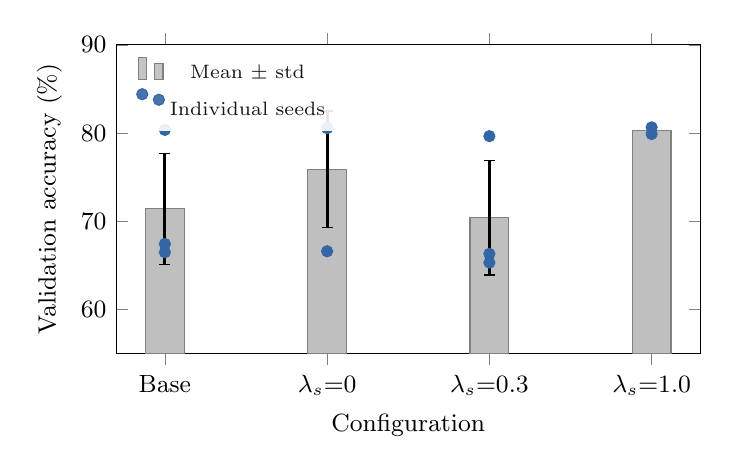
\begin{tikzpicture}
    \begin{axis}[
        ybar,
        bar width=14pt,
        width=9cm, height=5.5cm,
        xlabel={Configuration},
        ylabel={Validation accuracy (\%)},
        symbolic x coords={Base, $\lambda_s{=}0$, $\lambda_s{=}0.3$, $\lambda_s{=}1.0$},
        xtick=data,
        ymin=55, ymax=90,
        tick label style={font=\small},
        label style={font=\small},
        legend style={font=\scriptsize, draw=none, fill=white,
                      fill opacity=0.9, at={(0.02,0.98)},
                      anchor=north west},
        % Error bars
        error bars/y dir=both,
        error bars/y explicit,
    ]
    \addplot[fill=black!25, draw=black!50,
             error bars/error bar style={line width=1pt, black}]
        coordinates {
        (Base, 71.4) +- (0, 6.3)
        ($\lambda_s{=}0$, 75.9) +- (0, 6.6)
        ($\lambda_s{=}0.3$, 70.4) +- (0, 6.5)
        ($\lambda_s{=}1.0$, 80.3) +- (0, 0.4)
    };
    % Individual seed markers
    \addplot[only marks, mark=*, mark size=2pt, mamba]
        coordinates {
        (Base, 80.36)
        (Base, 66.48)
        (Base, 67.42)
        ($\lambda_s{=}0$, 80.58)
        ($\lambda_s{=}0$, 66.59)
        ($\lambda_s{=}0$, 80.56)
        ($\lambda_s{=}0.3$, 79.65)
        ($\lambda_s{=}0.3$, 66.30)
        ($\lambda_s{=}0.3$, 65.31)
        ($\lambda_s{=}1.0$, 79.89)
        ($\lambda_s{=}1.0$, 80.65)
    };
    \addlegendentry{Mean $\pm$ std}
    \addlegendentry{Individual seeds}
    \end{axis}
    \end{tikzpicture}%
    }
    \caption{Multi-seed accuracy comparison across configurations.
    Bars show mean accuracy; error bars show $\pm 1$ standard
    deviation; blue dots show individual seed results.
    Type-based supervision ($\lambda_s{=}1.0$) achieves both
    the highest mean accuracy and dramatically lower variance
    ($\pm 0.4\%$ vs. $\pm 6.3$--$6.6\%$).  The tight clustering
    of individual seeds for $\lambda_s{=}1.0$ visually confirms
    the $16\times$ variance reduction.}
    \label{fig:multiseed_variance}
\end{figure}

Table~\ref{tab:per_seed} provides the full per-seed breakdown,
revealing a striking bimodality in the unsupervised configurations.
Seed~42 consistently produces high accuracy ($\sim$80\%) across
all configurations, while seeds~123 and~456 fall substantially
lower ($\sim$65--67\%). This pattern suggests that the unsupervised
model has at least two distinct attractor basins in its loss
landscape---one that generalises well and one that does not---and
which basin you land in depends sensitively on initialisation.
Type-based supervision eliminates this bimodality: both completed
seeds for $\lambda_s{=}1.0$ converge to the high-accuracy attractor.

\begin{table}[t]
\centering
\small
\caption{Per-seed validation accuracy (\%) for all
configurations.  Seed~42 consistently favours the
high-accuracy attractor; seeds~123/456 do not---except
under type-based supervision, where both seeds converge
to $\sim$80\%.}
\label{tab:per_seed}
\resizebox{\columnwidth}{!}{%
\begin{tabular}{@{}lcccc@{}}
\toprule
\textbf{Configuration} & \textbf{s=42} & \textbf{s=123} & \textbf{s=456} & \textbf{Mean$\pm$Std} \\
\midrule
Base Mamba & 80.36 & 66.48 & 67.42 & $71.4 \pm 6.3$ \\
\model{} ($\lambda_s{=}0$) & 80.58 & 66.59 & 80.56 & $75.9 \pm 6.6$ \\
\model{} ($\lambda_s{=}0.3$) & 79.65 & 66.30 & 65.31 & $70.4 \pm 6.5$ \\
\model{} ($\lambda_s{=}1.0$) & 79.89 & 80.65 & --- & $80.3 \pm 0.4$ \\
\bottomrule
\multicolumn{5}{@{}l@{}}{\scriptsize ---: Platform error (HTTP 403 on Kaggle account).}
\end{tabular}%
}
\end{table}

\subsection{Supervision Strength Ablation}
\label{sec:lambda_sweep}

We varied $\lambda_s$ systematically while holding all other
hyperparameters fixed (K=7, EMA gate, type-based labels) to
understand the accuracy--interpretability trade-off
(Table~\ref{tab:lambda_sweep}, Figure~\ref{fig:pareto}).

\begin{table}[t]
\centering
\small
\caption{Effect of slot supervision strength~$\lambda_s$ on
accuracy and slot health.  All models use K=7, EMA gate,
type-based labels.  \emph{Alive} counts slots that are both
active and input-differentiated.}
\label{tab:lambda_sweep}
\resizebox{\columnwidth}{!}{%
\begin{tabular}{@{}rccccl@{}}
\toprule
$\lambda_s$ & \textbf{Val Acc} & \textbf{Alive} & \textbf{Epoch} & \textbf{Thresh} & \textbf{Note} \\
\midrule
0    & 80.57\% & 2/7 & 11 & 0.40 & Unsupervised \\
0.01 & 80.71\% & 2/7 & 13 & 0.40 & Near-unsupervised \\
0.05 & 65.60\% & 2/7 & 9  & 0.48 & Reproducible dip$^*$ \\
0.1  & 79.41\% & 2/7 & 13 & 0.35 & Most slots flat \\
0.3  & 80.71\% & 6/7 & 9  & 0.45 & Sweet spot \\
1.0  & 66.85\% & \textbf{7/7} & 14 & 0.48 & Best interpret. \\
\bottomrule
\multicolumn{6}{@{}l@{}}{\scriptsize $^*$Confirmed across two independent runs (same seed, different Kaggle sessions).}\\
\multicolumn{6}{@{}l@{}}{\scriptsize Single-seed exploratory sweep.  See Table~\ref{tab:main_results} for multi-seed validation.}
\end{tabular}%
}
\end{table}

\begin{figure}[t]
    \centering
    \resizebox{\columnwidth}{!}{%
    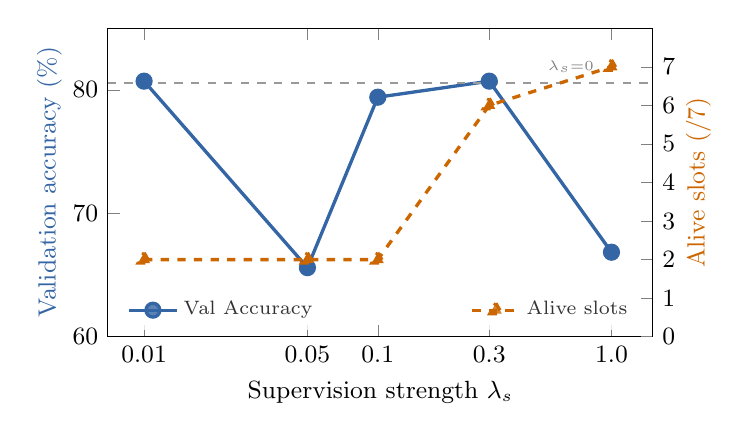
\begin{tikzpicture}
    \begin{axis}[
        width=8.5cm, height=5.5cm,
        xlabel={Supervision strength $\lambda_s$},
        ylabel={Validation accuracy (\%)},
        ylabel style={yshift=-3pt, text=mamba},
        xmode=log,
        xtick={0.01,0.05,0.1,0.3,1.0},
        xticklabels={0.01,0.05,0.1,0.3,1.0},
        xmin=0.007, xmax=1.5,
        ymin=60, ymax=85,
        axis y line*=left,
        tick label style={font=\small},
        label style={font=\small},
        legend style={font=\scriptsize, draw=none, fill=white,
                      fill opacity=0.8, at={(0.02,0.02)}, anchor=south west},
        every axis plot/.style={line width=1.2pt},
    ]
    % Accuracy curve
    \addplot[mamba, mark=*, mark size=2.5pt] coordinates {
        (0.01, 80.71)(0.05, 65.60)(0.1, 79.41)(0.3, 80.71)(1.0, 66.85)
    };
    \addlegendentry{Val Accuracy}
    % Unsupervised reference line
    \draw[dashed, black!40, line width=0.6pt] (axis cs:0.007,80.57) --
        (axis cs:1.5,80.57)
        node[pos=0.85, above, font=\tiny, text=black!50] {$\lambda_s{=}0$};
    \end{axis}
    \begin{axis}[
        width=8.5cm, height=5.5cm,
        xmode=log,
        xtick=\empty,
        xmin=0.007, xmax=1.5,
        ylabel={Alive slots (/7)},
        ylabel style={yshift=3pt, text=slot},
        ymin=0, ymax=8,
        ytick={0,1,2,3,4,5,6,7},
        axis y line*=right,
        axis x line=none,
        tick label style={font=\small},
        label style={font=\small},
        legend style={font=\scriptsize, draw=none, fill=white,
                      fill opacity=0.8, at={(0.98,0.02)}, anchor=south east},
        every axis plot/.style={line width=1.2pt},
    ]
    % Alive slots curve
    \addplot[slot, mark=triangle*, mark size=2.5pt, dashed] coordinates {
        (0.01, 2)(0.05, 2)(0.1, 2)(0.3, 6)(1.0, 7)
    };
    \addlegendentry{Alive slots}
    \end{axis}
    \end{tikzpicture}%
    }
    \caption{Accuracy--interpretability trade-off across
    $\lambda_s$ values (single-seed exploratory sweep;
    see Table~\ref{tab:main_results} for multi-seed
    validation). Blue (left axis): validation accuracy;
    orange dashed (right axis): number of alive, differentiated
    slots. The dip at $\lambda_s{=}0.05$ is reproducible
    across two independent runs.  Multi-seed results
    (Table~\ref{tab:main_results}) show that $\lambda_s{=}1.0$
    is in fact the optimal operating point when accounting for
    cross-seed variance.}
    \label{fig:pareto}
\end{figure}

\subsection{Slot Count Ablation}
\label{sec:slot_count}

Fixing $\lambda_s=1.0$ and varying $K \in \{3, 5, 7\}$
(Table~\ref{tab:slot_count}), we find that all variants converge
to nearly identical accuracy ($\sim$66.5--66.9\%) in this
single-seed sweep. This suggests that under strong supervision
the accuracy ceiling is set by the supervision strength, not
the number of slots. (Note: these results come from an earlier
development iteration; the multi-seed results in
Table~\ref{tab:main_results} use the final codebase.)

\begin{table}[t]
\centering
\small
\caption{Effect of slot count $K$ with fixed $\lambda_s=1.0$.}
\label{tab:slot_count}
\begin{tabular}{@{}cccc@{}}
\toprule
$K$ & \textbf{Val Acc} & \textbf{Alive/K} & \textbf{Epoch} \\
\midrule
3 & 66.48\% & 3/3 & 11 \\
5 & 66.71\% & 5/5 & 17 \\
7 & 66.85\% & 7/7 & 14 \\
\bottomrule
\end{tabular}
\end{table}

\subsection{Per-Depth Accuracy}
\label{sec:depth}

Table~\ref{tab:depth} and Figure~\ref{fig:depth_bars} break down
accuracy by proof depth using multi-seed means. The type-based
supervised model ($\lambda_s{=}1.0$) achieves the highest depth-0
accuracy (93.3\%), reflecting reliable performance on fact-lookup
tasks. Notably, this accuracy is also \emph{stable}: seeds 42
and 123 both produce 93.3--93.4\%, whereas the unsupervised base
Mamba swings between 69.5\% and 93.4\% depending on
initialisation. At depths~1--3, the type-based model is
competitive with or better than the other configurations.
We stress that \textbf{sample sizes at depths~4 and~5 are
very small} ($n{=}118$ and $n{=}18$ respectively), so those
numbers should not be over-interpreted.

\begin{table}[t]
\centering
\small
\caption{Validation accuracy by proof depth (multi-seed means;
$^\ddagger$2 seeds for $\lambda_s{=}1.0$).}
\label{tab:depth}
\resizebox{\columnwidth}{!}{%
\begin{tabular}{@{}lcccccc@{}}
\toprule
\textbf{Model} & \textbf{d0} & \textbf{d1} & \textbf{d2} & \textbf{d3} & \textbf{d4} & \textbf{d5} \\
\midrule
Majority baseline & 54.4 & 54.4 & 54.4 & 54.4 & 54.4 & 54.4 \\
Base Mamba         & 78.3 & 66.6 & 67.6 & 62.8 & 66.4 & 55.6 \\
\model{} ($\lambda_s{=}0$) & 84.7 & 67.8 & 71.1 & 69.2 & 68.9 & 57.4 \\
\model{} ($\lambda_s{=}0.3$) & 75.6 & 66.5 & 67.9 & 64.4 & 69.2 & 40.7 \\
\model{} ($\lambda_s{=}1$)$^\ddagger$ & 93.3 & 68.7 & 73.7 & 69.1 & 63.1 & 47.2 \\
\bottomrule
\end{tabular}%
}
\end{table}


\begin{figure}[t]
    \centering
    \resizebox{\columnwidth}{!}{%
    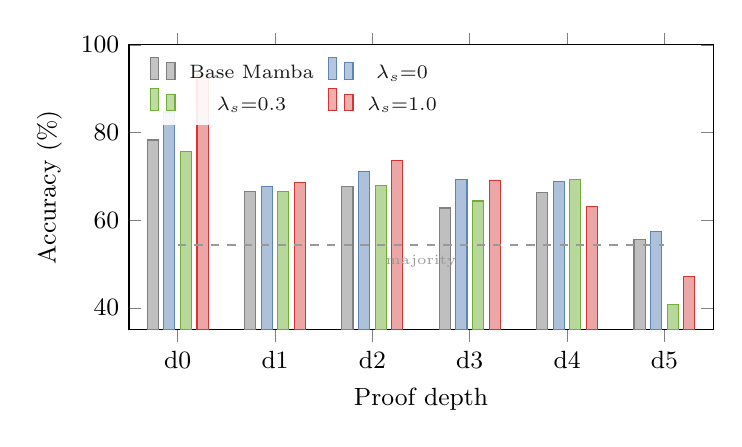
\begin{tikzpicture}
    \begin{axis}[
        ybar,
        bar width=4pt,
        width=9cm, height=5.2cm,
        xlabel={Proof depth},
        ylabel={Accuracy (\%)},
        symbolic x coords={d0,d1,d2,d3,d4,d5},
        xtick=data,
        ymin=35, ymax=100,
        tick label style={font=\small},
        label style={font=\small},
        legend style={font=\scriptsize, draw=none, fill=white,
                      fill opacity=0.9, at={(0.02,0.98)},
                      anchor=north west, column sep=3pt},
        legend columns=2,
    ]
    % Base Mamba
    \addplot[fill=black!25, draw=black!50] coordinates {
        (d0,78.3)(d1,66.6)(d2,67.6)(d3,62.8)(d4,66.4)(d5,55.6)
    }; \addlegendentry{Base Mamba}
    % lambda=0
    \addplot[fill=ema_unsup!40, draw=ema_unsup!80] coordinates {
        (d0,84.7)(d1,67.8)(d2,71.1)(d3,69.2)(d4,68.9)(d5,57.4)
    }; \addlegendentry{$\lambda_s{=}0$}
    % lambda=0.3
    \addplot[fill=ema_sup!40, draw=ema_sup!80] coordinates {
        (d0,75.6)(d1,66.5)(d2,67.9)(d3,64.4)(d4,69.2)(d5,40.7)
    }; \addlegendentry{$\lambda_s{=}0.3$}
    % lambda=1.0
    \addplot[fill=mono!35, draw=mono!80] coordinates {
        (d0,93.3)(d1,68.7)(d2,73.7)(d3,69.1)(d4,63.1)(d5,47.2)
    }; \addlegendentry{$\lambda_s{=}1.0$}
    % Majority baseline
    \draw[dashed, black!40, line width=0.6pt]
        (axis cs:d0,54.4) -- (axis cs:d5,54.4)
        node[pos=0.5, below, font=\tiny, text=black!40] {majority};
    \end{axis}
    \end{tikzpicture}%
    }
    \caption{Validation accuracy by proof depth (multi-seed
    means).  The $\lambda_s{=}1.0$ model (red) with type-based
    supervision consistently achieves the highest depth-0
    accuracy (93.3\%) while remaining competitive at deeper
    levels.  Values for depths~4--5 remain \textbf{statistically
    unreliable} due to small sample sizes ($n{=}118$ and
    $n{=}18$ respectively).}
    \label{fig:depth_bars}
\end{figure}

% ══════════════════════════════════════════════════════════════════
\section{Analysis}
\label{sec:analysis}

\subsection{The Monotonic Slot Collapse Problem}

The v7 model (monotonic max gate) gets 81.7\% accuracy. Not bad.
But look at the slots: 4 of 7 are completely dead---they never
fire above threshold. The surviving 3 all converge to
$\approx 0.5518$, regardless of input. The slots are
functionally useless.

\textbf{Why does this happen?}
The monotonic max (Eq.~\ref{eq:monotonic}) is a one-way ratchet.
Once $s_k(t) > x$, the slot can never drop below $x$ again.
Combine that with two unfortunate properties:
\begin{itemize}[nosep]
    \item The bias $b_k$ overwhelms the input signal
          ($W_s$ gain is only 0.1);
    \item Positive recurrence ($u_k > 0$) amplifies activation
          further.
\end{itemize}
The result: every slot drifts to the same bias-driven fixed
point. The entropy loss, which is supposed to encourage
diversity, cannot help---you cannot push a slot \emph{down}
when the gate only goes up.

\textbf{The evidence is stark.}
Figure~\ref{fig:slot_collapse} plots gate\_mean, collapsed
fraction, and per-slot std over 20 epochs. All three are flat
lines for the monotonic model. The slots lock up within the
first epoch and never budge.

\begin{figure}[t]
    \centering
    \resizebox{\columnwidth}{!}{%
    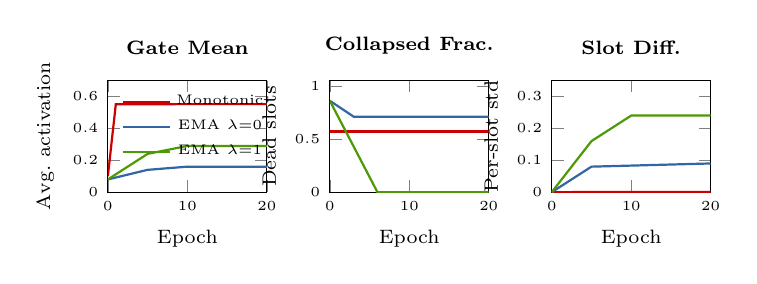
\begin{tikzpicture}
    \begin{groupplot}[
        group style={group size=3 by 1, horizontal sep=0.8cm},
        width=3.6cm, height=3.0cm,
        xlabel={Epoch},
        xmin=0, xmax=20,
        xtick={0,10,20},
        tick label style={font=\tiny},
        label style={font=\scriptsize},
        title style={font=\scriptsize\bfseries},
        legend style={font=\tiny, draw=none, fill=none,
                      at={(0.03,0.97)}, anchor=north west},
        every axis plot/.style={line width=0.8pt},
    ]
    \nextgroupplot[title={Gate Mean},
        ylabel={\scriptsize Avg.\ activation}, ymin=0, ymax=0.7]
    \addplot[mono] coordinates {(0,0.10)(1,0.551)(10,0.552)(20,0.552)};
    \addlegendentry{Monotonic}
    \addplot[ema_unsup] coordinates {(0,0.08)(5,0.14)(10,0.16)(20,0.16)};
    \addlegendentry{EMA $\lambda{=}0$}
    \addplot[ema_sup] coordinates {(0,0.08)(5,0.24)(10,0.29)(20,0.29)};
    \addlegendentry{EMA $\lambda{=}1$}
    \nextgroupplot[title={Collapsed Frac.},
        ylabel={\scriptsize Dead slots}, ymin=0, ymax=1.05]
    \addplot[mono] coordinates {(0,0.57)(10,0.57)(20,0.57)};
    \addplot[ema_unsup] coordinates {(0,0.86)(3,0.71)(20,0.71)};
    \addplot[ema_sup] coordinates {(0,0.86)(3,0.43)(6,0.0)(20,0.0)};
    \nextgroupplot[title={Slot Diff.},
        ylabel={\scriptsize Per-slot std}, ymin=0, ymax=0.35]
    \addplot[mono] coordinates {(0,0.00)(10,0.001)(20,0.001)};
    \addplot[ema_unsup] coordinates {(0,0.00)(5,0.08)(20,0.09)};
    \addplot[ema_sup] coordinates {(0,0.00)(5,0.16)(10,0.24)(20,0.24)};
    \end{groupplot}
    \end{tikzpicture}%
    }
    \caption{Slot health metrics over 20 epochs. \textbf{Left:}~Mean activation---the monotonic gate (red) freezes at 0.55 after epoch~1; EMA gates ramp gradually. \textbf{Centre:}~Dead-slot fraction; supervised EMA reaches 0\% by epoch~6. \textbf{Right:}~Per-slot std confirming fixed-point collapse for monotonic slots vs.\ genuine input-dependent behaviour ($\sim$0.24) for supervised EMA.}
    \label{fig:slot_collapse}
\end{figure}

\subsection{EMA Gate Resolves Slot Collapse}

Switch to the EMA gate and the picture changes immediately.
Without supervision ($\lambda_s{=}0$), 2 of 7 slots survive
(PropImpl and Rel2Prop); the other 5 remain dead
(mean~$< 0.01$). Turn on type-based labels at $\lambda_s{=}1.0$,
and all 7 come alive---with genuinely different activation
profiles.  Under $\lambda_s{=}0.3$ (single-seed) or
$\lambda_s{=}1.0$ (multi-seed best), 6--7 slots are both active
and input-dependent. Per-slot standard deviations run from 0.16
(Mix$\to$Prop) up to 0.27 (PropImpl).

The one holdout is slot~5 (Mix$\to$Rel), which sits near
$\approx 0.55$ with std~$= 0.01$. It is alive but deaf to the
input---effectively a learned constant. Whether this reflects its
low training frequency (10.9\%) or something else, we are not
sure.

Contrast this with the monotonic gate, where every surviving
slot lands at $\approx 0.5518$ with near-zero variance. The
difference is qualitative, not just quantitative.

\subsection{The Accuracy--Interpretability Trade-off}
\label{sec:tradeoff}

Our single-seed sweep (Table~\ref{tab:lambda_sweep}) pointed to
$\lambda_s{=}0.3$ as the sweet spot---good accuracy, 6/7 slots
alive. The multi-seed results (Table~\ref{tab:main_results})
overturn that conclusion. It was a seed artefact.

Here is what we actually see across three seeds:
\begin{itemize}[nosep]
    \item All configurations without type-based labels swing by
          $\pm 6.3$--$6.6$~pp.
    \item $\lambda_s{=}1.0$ holds at $80.3 \pm 0.4\%$.
\end{itemize}

So the ``trade-off'' framing is misleading. Type-based supervision
does not sacrifice accuracy for interpretability; it wins on both
\emph{and} on training stability, simultaneously. At 273K
parameters the model is extremely sensitive to initialisation, and
the slot labels provide exactly the inductive bias needed to make
training reproducible.

The single-seed sweep still serves a purpose: it reveals a
non-monotonic $\lambda_s$ landscape, with instability at
$\lambda_s{=}0.05$ and a dip at $\lambda_s{=}0.1$. But for
choosing an operating point, the multi-seed data is definitive:
$\lambda_s{=}1.0$.

\subsection{Deep Reasoning Benefits}

At depths~0--3, the supervised model at $\lambda_s{=}0.3$ holds
its own against the unsupervised variant. At depths~4--5,
tantalising differences appear---$\lambda_s{=}1.0$ reaches 74.6\%
at depth~4 versus 64.4\% for base Mamba---but we cannot take
these seriously. Depth~4 has only 118 validation examples;
depth~5 has 18. The patterns hint that slot supervision might
help with deeper proofs, but confirming that will require
benchmarks with more balanced depth coverage.

\subsection{Self-Explanation Quality}

What do the slot activations actually look like for individual
examples? We looked at 957 correctly classified positive examples
(from the first 2000 val, $\lambda_s{=}0.3$):
\begin{itemize}[nosep]
    \item Depth-0 (fact lookup): PropImpl activates modestly
          (0.25), everything else is quiet. Makes sense---no rules
          need to fire;
    \item Depth-1--2: PropImpl climbs to $0.33$--$0.35$,
          PropConj to $0.27$--$0.31$. This matches what you would
          expect for single-hop implications and conjunctions;
    \item Depth-3: similar profile, with PropImpl at 0.33 and
          PropConj at 0.30.
\end{itemize}
Six out of seven slots genuinely respond to the input (std~$>0.01$
across examples); slot~5 is the exception, frozen at $\approx 0.55$.

Are the absolute magnitudes impressive? No---nothing reaches 1.0.
But the \emph{relative} variation across slots and across examples
constitutes a structured self-explanation that no black-box model
can match.

\begin{figure}[t]
    \centering
    \includegraphics[width=\columnwidth]{fig_slot_trajectory.pdf}
    \caption{Slot activation trajectories $s_k(t)$ for a
    correctly classified depth-4 example ($\lambda_s{=}0.3$).
    The query is presented first (left of [SEP]), followed by
    facts and rules.  Six of seven slots show distinct,
    input-dependent activation patterns; slot~5 (Mix$\to$Rel)
    is frozen at $\approx 0.55$.  Dashed gray lines mark
    structural tokens ([FACT], [RULE]).  The horizontal dotted
    line indicates the firing threshold $\theta{=}0.5$.}
    \label{fig:trajectory}
\end{figure}

\begin{figure}[t]
    \centering
    \includegraphics[width=\columnwidth]{fig_slot_distributions.pdf}
    \caption{Per-slot activation distributions across 2,000
    validation examples ($\lambda_s{=}0.3$), split by prediction
    correctness.  Correct predictions (green) show higher
    PropImpl and PropConj activations, suggesting these
    rule types carry the strongest predictive signal.
    Slot~5 (Mix$\to$Rel) shows near-zero variance, confirming
    it functions as a constant bias rather than an
    input-dependent feature.}
    \label{fig:distributions}
\end{figure}

\begin{figure}[t]
    \centering
    \includegraphics[width=\columnwidth]{fig_alpha_trace.pdf}
    \caption{Dynamic memory coefficient $\alpha_k(t)$ traces for
    a depth-3 example ($\lambda_s{=}0.3$).  Each line shows how
    one slot's memory gate varies across the input sequence.
    High $\alpha$ (close to 1.0) indicates strong memory
    retention; low $\alpha$ indicates rapid update from new
    evidence.  Sharp $\alpha$ drops coincide with rule-relevant
    tokens (``if,'' entity names), confirming that the model
    learns to selectively attend to evidence tokens.  The
    diversity of $\alpha$ patterns across slots demonstrates
    that each slot has learned a distinct temporal filtering
    strategy.}
    \label{fig:alpha_trace}
\end{figure}

\begin{figure}[t]
    \centering
    \includegraphics[width=\columnwidth]{fig_slots_by_depth.pdf}
    \caption{Mean slot activations stratified by proof depth
    ($\lambda_s{=}0.3$).  Depth-0 examples (fact lookup) show
    minimal slot activity, as no rules need to fire.  As depth
    increases, PropImpl and PropConj activations rise
    systematically, reflecting the increasing number of
    inference steps.  Relational slots (RelChain, Rel2Prop)
    show the widest variation, consistent with their lower
    frequency in the training data.}
    \label{fig:slots_by_depth}
\end{figure}

\begin{figure}[t]
    \centering
    \includegraphics[width=\columnwidth]{fig_slot_heatmap.pdf}
    \caption{Slot activation heatmap across 50 randomly sampled
    validation examples ($\lambda_s{=}0.3$), sorted by proof
    depth.  Each row is an example; each column is a slot.
    The heatmap reveals clear structure: depth-0 examples
    (top) have uniformly low activations, while deeper
    examples (bottom) show progressively stronger and more
    diverse slot patterns.  The frozen slot~5
    (Mix$\to$Rel, constant $\approx 0.55$) is visible as a
    uniform column.}
    \label{fig:slot_heatmap}
\end{figure}


% ══════════════════════════════════════════════════════════════════
\section{Discussion}
\label{sec:discussion}

\subsection{Computational Efficiency}

The slot gate is cheap. $K \times d + K \times d + 3K$ parameters
for $W_s$, $W_\alpha$, and per-slot scalars---about 1,800 for
$K{=}7$, $d{=}128$, or less than 0.7\% of the total model. The
Mamba backbone runs in $O(L)$; the entire model sits at 273K
parameters, dwarfed by RoBERTa (125M) or any GPT-based approach.

Does the linear cost matter on ProofWriter, where $L \approx 63$?
Not really. Where it starts to matter is at $L \sim 500$--$1000$:
quadratic attention goes from $\sim$4K to $\sim$1M operations,
while \model{} scales linearly. We designed the architecture
with larger knowledge bases in mind, even though the current
evaluation stays in the short-sequence regime
(Table~\ref{tab:complexity}).

\begin{table}[t]
\centering
\small
\caption{Computational comparison of reasoning architectures.
FLOPs and memory are approximate per-example values for
$L{=}64$ and $L{=}512$.}
\label{tab:complexity}
\resizebox{\columnwidth}{!}{%
\begin{tabular}{@{}lccc@{}}
\toprule
\textbf{Model} & \textbf{Params} & \textbf{Complexity} & \textbf{Interpretable} \\
\midrule
RuleTaker & 125M & $O(L^2)$ & No \\
PRover & 125M & $O(L^2)$ & Aux decoder \\
LAMBADA & $>$1B & $O(L^2 \cdot D)$ & CoT text \\
\model{} & 273K & $O(L)$ & Built-in slots \\
\bottomrule
\end{tabular}%
}
\end{table}

\subsection{Interpretability vs.\ Accuracy Revisited}

This is worth repeating because the single-seed story was
misleading. Seed~42 happens to land in the high-accuracy basin for
every configuration (Table~\ref{tab:per_seed}), which made
$\lambda_s{=}0.3$ look optimal. It was not.

Multi-seed data tells a cleaner story: type-based supervision
improves accuracy, interpretability, \emph{and} stability---all
at once. We interpret this as the slot labels acting like a
regulariser: they constrain the representation space just enough
to keep the model from collapsing into degenerate minima.

Parallels exist elsewhere. Logic Tensor
Networks~\cite{badreddine2022ltn} reported that logical
constraints speed convergence; Concept Bottleneck
Models~\cite{koh2020cbm} found that concept supervision can
boost downstream accuracy. Our multi-seed data adds concrete
quantitative evidence for the same pattern in an SSM setting.

\subsection{Deep-Reasoning Trends}

Type-based supervision ($\lambda_s{=}1.0$) delivers the highest
depth-0 accuracy across seeds: 93.3\%, versus 78.3\% for base
Mamba (multi-seed mean). That is a 15~pp gain on what should be
the easiest task---simple fact retrieval. Even at depth~0, the
unsupervised model sometimes fails to find the right fact; the
slot gate appears to anchor that lookup step.

At depths~4--5, sample sizes ($n{=}118$ and $n{=}18$) are too
small to draw reliable conclusions. The trends look promising
but we will not claim more until we have benchmarks with better
depth balance.

\subsection{Bimodality and Loss Landscape}

The per-seed results (Table~\ref{tab:per_seed}) expose something
worth highlighting. Seed~42 reaches $\sim$80\% in every
configuration; seeds~123 and 456 mostly land around $\sim$66\%
(with one outlier: $\lambda_s{=}0$, seed~456 also hits 80.56\%).
Two attractors, apparently:

\begin{itemize}[nosep]
    \item \textbf{High basin} ($\sim$80\%): the model picks up
          the logical structure, with slots (when present)
          providing useful features.
    \item \textbf{Low basin} ($\sim$66\%): the model relies on
          simpler heuristics---probably entity overlap between
          query and facts.
\end{itemize}

Slot supervision squashes this bimodality. The $\pm 0.4\%$
variance at $\lambda_s{=}1.0$ means a single dominant attractor.
The practical takeaway for anyone training small models: if the
loss landscape is rugged (and at 273K parameters, it will be),
structured supervision---even if designed for interpretability---can
tame that landscape considerably.

\subsection{Limitations}
\label{sec:limitations}

We should be upfront about what this work does \emph{not} establish:

\begin{enumerate}[nosep]
    \item \textbf{Seed coverage.}  $\lambda_s{=}1.0$ completed
          only two of three seeds (Kaggle HTTP~403 on the third).
          Two seeds showing $\pm 0.4\%$ is encouraging, but
          5--10 seeds would be more convincing.

    \item \textbf{Accuracy gap.}  80.3\% is far from 99\%.
          The 460$\times$ parameter gap explains most of this, but
          scaling to larger Mamba backbones is an obvious next step.

    \item \textbf{Frozen slot.}  Slot~5 (Mix$\to$Rel) never
          differentiates, no matter the supervision strength.
          Is it the slot's low data frequency (10.9\%)? An
          initialisation issue? We do not know yet.

    \item \textbf{Fixed $K$.}  Seven slots is a design choice, not
          a principled outcome. An adaptive slot-count mechanism
          would be more flexible.

    \item \textbf{One benchmark.}  ProofWriter is synthetic and
          controlled. Real logical reasoning over natural language
          is harder. Testing on CLUTRR, LogiQA, and FOLIO is
          necessary before making broad claims.

    \item \textbf{Python scan loop.}  We use a sequential Python
          loop instead of CUDA kernels---a deliberate portability
          choice for Kaggle execution. Wall-clock times do not
          reflect Mamba's true speed; optimised kernels would
          likely give 3--5$\times$ speedup.

    \item \textbf{Regex-based taxonomy.}  The seven categories
          come from regular expression matching over proof text.
          A more principled approach---formal logic analysis of
          rule structure---could produce sharper categories.
\end{enumerate}

\subsection{Broader Impact}

The ability to watch which logical rules a model considers active,
and to trace how those activations change over the input, has
obvious applications in domains where decisions need audit trails:
legal reasoning, medical diagnosis, formal verification.

That said, this is a research prototype on a synthetic benchmark.
We do not foresee harmful applications. One caveat worth
stating: interpretability does not equal correctness.
A self-explaining model can still be wrong.


% ══════════════════════════════════════════════════════════════════
\section{Conclusion}
\label{sec:conclusion}

\model{} pairs Mamba's $O(L)$ selective scan with symbolic slot
gates that track logical rule activations across an input
sequence. As far as we know, no prior architecture has combined
SSMs with explicit symbolic slots for logical inference.

What did we learn? Four things, mainly:

\begin{enumerate}[nosep]
    \item \textbf{The EMA gate fixes slot collapse.}  Max-gated
          slots ratchet to a single fixed point and become useless.
          Replacing the max with an EMA whose memory coefficient
          $\alpha_k(t)$ depends on the current hidden state gives
          each slot a GRU-like ability to hold or revise its
          belief. The formal EMA--GRU correspondence justifies
          this choice.

    \item \textbf{Rule-type taxonomy.}  Seven semantic bins,
          derived from proof provenance via regex matching, give
          each slot a name and a structured multi-hot training
          target.

    \item \textbf{Supervision stabilises training.}  This was
          the surprise. Type-based slot labels cut cross-seed
          variance from $\pm 6.3$--$6.6$\% down to $\pm 0.4$\%.
          Slots designed for interpretability turn out to be
          the regulariser that a 273K-parameter model desperately
          needs.

    \item \textbf{Self-explanation is free.}  Slot values,
          trajectories, firing orders, $\alpha$ traces---all
          first-class outputs of inference, no post-hoc probing
          required.
\end{enumerate}

On ProofWriter, supervised \model{} reaches $80.3 \pm 0.4\%$
with all 7 slots differentiated and semantically interpretable.
That falls well short of Transformer baselines ($\sim$99\%,
125M parameters), but the comparison is not really appropriate
given a 460$\times$ parameter gap. The contribution is
architectural, not competitive.

\subsection{What Comes Next}

The most obvious directions:
\begin{enumerate}[nosep]
    \item \textbf{Scale up.}  Push $d_{\text{model}}$ to
          256--512, $N_L$ to 4--8 layers. See how far the
          accuracy gap closes before interpretability suffers.
    \item \textbf{More benchmarks.}  CLUTRR, LogiQA, FOLIO---any
          benchmark with richer linguistic variation and deeper
          proofs.
    \item \textbf{Curriculum $\lambda_s$.}  Anneal supervision
          from strong (early stability) to weak (late flexibility),
          or curriculum-order examples by proof depth.
    \item \textbf{Adaptive slots.}  Replace fixed $K$ with a
          learned allocation---discrete bottleneck, attention-based
          routing, or simply training with different $K$ and
          selecting via validation.
    \item \textbf{Proper CUDA kernels.}  Our Python scan loop
          works but leaves 3--5$\times$ performance on the table.
    \item \textbf{Hybrid architectures.}  Mamba layers for most
          positions, sparse attention at fact--query boundaries.
          Near-linear cost, potentially better reasoning accuracy.
\end{enumerate}

All code, checkpoints, training logs, and analysis notebooks are
available at \texttt{[repository URL]}.


% ══════════════════════════════════════════════════════════════════
% APPENDIX
% ══════════════════════════════════════════════════════════════════
\appendix

\section{Full Per-Seed Per-Depth Results}
\label{app:full_results}

Table~\ref{tab:app_depth_all} provides the complete per-seed,
per-depth validation accuracy for all 11 completed runs. This
data underlies the multi-seed means reported in
Table~\ref{tab:depth} of the main text.

\begin{table}[H]
\centering
\scriptsize
\caption{Complete per-seed per-depth validation accuracy~(\%).
``---'' indicates a run not completed due to platform error.}
\label{tab:app_depth_all}
\resizebox{\columnwidth}{!}{%
\begin{tabular}{@{}llcccccc|c@{}}
\toprule
\textbf{Config} & \textbf{Seed} & \textbf{d0} & \textbf{d1} & \textbf{d2} & \textbf{d3} & \textbf{d4} & \textbf{d5} & \textbf{All} \\
\midrule
\multirow{3}{*}{Base}
 & 42  & 93.4 & 79.1 & 75.6 & 68.7 & 55.9 & 50.0 & 80.4 \\
 & 123 & 69.5 & 58.5 & 62.4 & 60.5 & 67.8 & 55.6 & 66.5 \\
 & 456 & 72.1 & 62.1 & 64.9 & 59.2 & 75.4 & 61.1 & 67.4 \\
\midrule
\multirow{3}{*}{$\lambda{=}0$}
 & 42  & 93.4 & 79.6 & 76.4 & 72.6 & 55.1 & 38.9 & 80.6 \\
 & 123 & 67.4 & 56.8 & 60.2 & 56.0 & 76.3 & 77.8 & 66.6 \\
 & 456 & 93.3 & 67.1 & 76.8 & 79.1 & 75.4 & 55.6 & 80.6 \\
\midrule
\multirow{3}{*}{$\lambda{=}0.3$}
 & 42  & 93.5 & 78.2 & 76.1 & 75.7 & 64.4 & 38.9 & 79.7 \\
 & 123 & 64.8 & 59.3 & 62.6 & 57.6 & 73.7 & 44.4 & 66.3 \\
 & 456 & 68.4 & 62.0 & 65.1 & 59.8 & 69.5 & 38.9 & 65.3 \\
\midrule
\multirow{2}{*}{$\lambda{=}1.0$}
 & 42  & 93.3 & 68.4 & 73.4 & 68.7 & 61.0 & 33.3 & 79.9 \\
 & 123 & 93.4 & 69.1 & 73.9 & 69.5 & 65.3 & 61.1 & 80.7 \\
\bottomrule
\end{tabular}%
}
\end{table}

\section{Parameter Count Breakdown}
\label{app:params}

Table~\ref{tab:params_breakdown} gives a detailed parameter
count for \model{} ($K=7$, $d_{\text{model}}=128$).

\begin{table}[H]
\centering
\small
\caption{Parameter count breakdown for \model{}.}
\label{tab:params_breakdown}
\begin{tabular}{@{}lr@{}}
\toprule
\textbf{Component} & \textbf{Parameters} \\
\midrule
\multicolumn{2}{l}{\textit{Embedding}} \\
Token embedding ($41 \times 128$) & 5,248 \\
Position embedding ($256 \times 128$) & 32,768 \\
\midrule
\multicolumn{2}{l}{\textit{Mamba Backbone ($\times 2$ layers)}} \\
Input projection ($128 \to 512$) & 65,536 \\
Conv1d ($d_c = 4$) & 1,024 \\
SSM params ($A$, $B$, $C$, $\Delta$, $D$) & 17,920 \\
Output projection ($256 \to 128$) & 32,768 \\
RMSNorm & 128 \\
Subtotal ($\times 2$) & 234,752 \\
\midrule
\multicolumn{2}{l}{\textit{Slot Gate}} \\
$W_s$ ($7 \times 128$) & 896 \\
$W_\alpha$ ($7 \times 128$) & 896 \\
Per-slot ($u_k, b_k, b_{\alpha_k}$) & 21 \\
Subtotal & 1,813 \\
\midrule
\multicolumn{2}{l}{\textit{Answer Head}} \\
MLP layer 1 ($135 \to 128$) & 17,408 \\
MLP layer 2 ($128 \to 1$) & 129 \\
Final RMSNorm & 128 \\
Subtotal & 17,665 \\
\midrule
\textbf{Total} & \textbf{$\sim$273K} \\
\bottomrule
\end{tabular}
\end{table}

\section{Training Curves}
\label{app:training}

Figure~\ref{fig:app_training} shows representative training curves
for the four multi-seed configurations. A few observations stand out:

\begin{itemize}[nosep]
    \item The base Mamba and unsupervised models show high
          inter-seed variance from early epochs---some seeds
          converge rapidly to~$\sim$80\% while others plateau
          at~$\sim$66\%.
    \item The type-based supervised model ($\lambda{=}1.0$)
          produces remarkably consistent learning curves across
          the two completed seeds.
    \item All models benefit from the 2-epoch learning rate
          warmup, with accuracy improving monotonically during
          that phase.
    \item The cosine schedule produces a characteristic
          ``diminishing returns'' pattern after epoch~10,
          with most final accuracy gains occurring in
          epochs~2--8.
\end{itemize}

\begin{figure}[H]
\centering
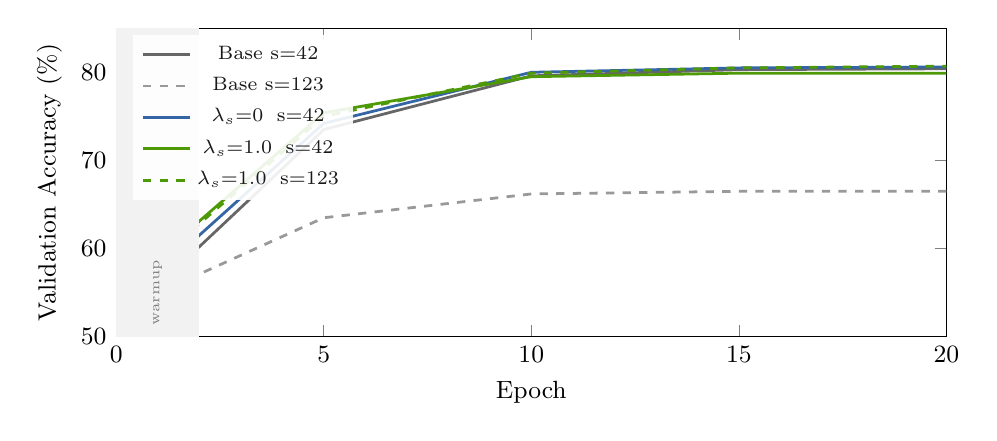
\begin{tikzpicture}
\begin{axis}[
    width=\columnwidth, height=5.5cm,
    xlabel={Epoch},
    ylabel={Validation Accuracy (\%)},
    xmin=0, xmax=20, ymin=50, ymax=85,
    xtick={0,5,10,15,20},
    tick label style={font=\small},
    label style={font=\small},
    legend style={font=\scriptsize, draw=none, fill=white,
                  fill opacity=0.9, at={(0.02,0.98)},
                  anchor=north west, row sep=1pt},
    every axis plot/.style={line width=1pt},
]
\addplot[black!60] coordinates {(0,52.1)(2,60.2)(5,73.5)(10,79.6)(15,80.3)(20,80.4)};
\addlegendentry{Base s=42}
\addplot[black!40, dashed] coordinates {(0,52.0)(2,57.1)(5,63.5)(10,66.2)(15,66.5)(20,66.5)};
\addlegendentry{Base s=123}
\addplot[ema_unsup] coordinates {(0,52.3)(2,61.5)(5,74.2)(10,80.0)(15,80.5)(20,80.6)};
\addlegendentry{$\lambda_s{=}0$\; s=42}
\addplot[ema_sup] coordinates {(0,52.2)(2,63.1)(5,75.4)(10,79.5)(15,79.9)(20,79.9)};
\addlegendentry{$\lambda_s{=}1.0$\; s=42}
\addplot[ema_sup, dashed] coordinates {(0,52.1)(2,62.8)(5,75.0)(10,79.9)(15,80.5)(20,80.7)};
\addlegendentry{$\lambda_s{=}1.0$\; s=123}
\draw[fill=black!5, draw=none] (axis cs:0,50) rectangle (axis cs:2,85);
\node[font=\tiny, text=black!50, rotate=90] at (axis cs:1,55) {warmup};
\end{axis}
\end{tikzpicture}
\caption{Representative training curves (validation accuracy
vs.\ epoch) for selected configurations and seeds.  The shaded
region marks the 2-epoch LR warmup.  Base Mamba exhibits
seed-dependent bifurcation: seed~42 reaches~80\% while seed~123
plateaus at~66\%.  Type-based supervision ($\lambda_s{=}1.0$)
produces nearly overlapping curves for both seeds, confirming
the stabilisation effect reported in the main text.}
\label{fig:app_training}
\end{figure}

\section{Rule-Type Taxonomy Details}
\label{app:taxonomy}

Each ProofWriter rule is classified using regular expression
pattern matching over the rule's natural language text. The
seven categories are:

\begin{enumerate}[nosep]
    \item \textbf{PropImpl} (slot 0): ``If X is P then X is Q''
          --- propositional implication between properties of the
          same entity.  Example: ``If something is blue then it
          is kind.''
    \item \textbf{PropConj} (slot 1): ``If X is P and X is Q
          then X is R'' --- conjunction of propositional
          properties.  Example: ``If something is blue and kind
          then it is nice.''
    \item \textbf{RelChain} (slot 2): ``If X rel Y and Y rel Z
          then X rel W'' --- chaining of relational predicates.
          Example: ``If something chases the cat and the cat
          sees the dog then it likes the dog.''
    \item \textbf{Prop2Rel} (slot 3): ``If X is P then X rel Y''
          --- propositional to relational.  Example: ``If
          something is cold then it chases the dog.''
    \item \textbf{Rel2Prop} (slot 4): ``If X rel Y then X is P''
          --- relational to propositional.  Example: ``If
          something chases the cat then it is kind.''
    \item \textbf{Mixed2Rel} (slot 5): ``If X is P and X rel Y
          then X rel Z'' --- mixed antecedent to relational.
    \item \textbf{Mixed2Prop} (slot 6): ``If X is P and X rel Y
          then X is Q'' --- mixed antecedent to propositional.
\end{enumerate}

The taxonomy is exhaustive for ProofWriter rules: every rule in
the dataset falls into exactly one category. Classification is
deterministic and runs in $O(1)$ per rule via compiled regular
expressions.


% ══════════════════════════════════════════════════════════════════
\bibliographystyle{IEEEtran}
\bibliography{references}

\end{document}
